%==================================
% SMDS TEMPLATE 
%==================================
% This document is a simplified template for preparing manuscripts for the Statistical Modeling and Data Science (SMDS) journal. The template provides basic structural elements for article preparation, including metadata, author affiliations, equations, tables, figures, and references. Authors may adapt this template to suit the requirements of their manuscript.

\documentclass[11pt,twoside]{article}

%==================================
% PACKAGES
%==================================
\usepackage{titlesec}
\titlespacing*{\section}{0pt}{1.5ex plus 0.5ex minus 0.2ex}{0.8ex plus 0.2ex}
\titlespacing*{\subsection}{0pt}{1.2ex plus 0.5ex minus 0.2ex}{0.5ex plus 0.2ex}

\usepackage[utf8]{inputenc}
\usepackage{amsmath,amssymb}
\usepackage[T1]{fontenc}
\usepackage{lmodern}
\usepackage{graphicx}
\usepackage{geometry}
\geometry{margin=1in}
\usepackage{booktabs}
\usepackage{array}
\usepackage{tabularx}
\usepackage{longtable}
\usepackage{adjustbox}
\usepackage{float}
\usepackage{caption}
\usepackage{placeins}
\usepackage{subcaption}
\usepackage{csquotes}
\usepackage[
backend=biber,
style=numeric-comp,
sorting=none,
giveninits=true,
doi=true,
url=true
]{biblatex}
\addbibresource{SMDSBib.bib}
\usepackage{fancyhdr}
\newcommand{\shorttitle}{}
\newcommand{\shortauthor}{}
\pagestyle{fancy}
\fancyhf{}
\fancyhead[L]{\small\shorttitle}
\fancyhead[R]{\small\shortauthor}
\fancyfoot[C]{\thepage}

\usepackage[colorlinks=true,allcolors=blue]{hyperref}
\newcommand{\orcidlink}[1]{%
\href{https://orcid.org/#1}{
\includegraphics[height=1.6ex]{ORCID_iD.png}}%
}

\graphicspath{{figures_pdf/}}
\captionsetup{font=small,labelfont=bf}
\setlength{\parindent}{1.2em}
\setlength{\parskip}{0.25em}
\sloppy

%==================================
% SIMPLE SMDS MACROS (Compatibility Layer)
%==================================

\newcommand{\SMDStitle}[1]{\title{\bfseries #1}}
\newcommand{\SMDSshorttitle}[1]{\def\shorttitle{#1}}
\newcommand{\SMDSshortafill}[1]{\def\shortauthor{#1}}

\newcommand{\SMDSaffilone}[1]{\def\affilone{#1}}
\newcommand{\SMDSaffiltwo}[1]{\def\affiltwo{#1}}
\newcommand{\SMDSaffilthree}[1]{\def\affilthree{#1}}
\newcommand{\SMDSaffilfour}[1]{\def\affilfour{#1}}
\newcommand{\SMDSaffilfive}[1]{\def\affilfive{#1}}

\newcommand{\SMDSauthorone}[4]{\def\authorone{#1$^{#2}$\,\orcidlink{#3}}}
\newcommand{\SMDSauthortwo}[4]{\def\authortwo{#1$^{#2}$\,\orcidlink{#3}}}
\newcommand{\SMDSauthorthree}[4]{\def\authorthree{#1$^{#2}$\,\orcidlink{#3}}}
\newcommand{\SMDSauthorfour}[4]{\def\authorfour{#1$^{#2}$\,\orcidlink{#3}}}
\newcommand{\SMDSauthorfive}[4]{\def\authorfive{#1$^{#2}$\,\orcidlink{#3}}}
\newcommand{\SMDSauthorsix}[4]{\def\authorsix{#1$^{#2}$\,\orcidlink{#3}}}

\newcommand{\SMDScorrespoding}[2]{%
\def\corrauthor{#1 \href{mailto:#2}{#2}}}

\newcommand{\SMDSKeywords}[1]{
\vspace{0.5em}
\noindent\textbf{Keywords:} #1
}

\newcommand{\acknowledg}[1]{
\section*{Acknowledgments}
#1
}

\newcommand{\funding}[1]{
\section*{Funding}
#1
}


%==================================
% METADATA
%==================================

\SMDStitle{Comparative Explainable Ensemble Learning for Flood Susceptibility Mapping Using Sentinel-1-Derived Flood Inventory and Multi-Source Geospatial Data: A Case Study of the Semarang-Demak Coastal Area
}

\SMDSshortafill{M. I. A. Hakim et al.}
\SMDSshorttitle{Flood Susceptibility Mapping}

\SMDSaffilone{Department of Statistics and Data Science, Faculty of Mathematics and Natural Sciences, Universitas Negeri Semarang, Indonesia}


%----------------------------------
% AUTHORS
%----------------------------------
% Each author must provide a valid ORCID iD (16-digit format).
% Register at: https://orcid.org/register
% Format: \SMDSauthorX{Name}{AffiliationID}{ORCID}{email}

\SMDSauthorone{M Irfan Al Hakim}{1}{0009-0005-1222-7960}
{mirfanhakim25@students.unnes.ac.id}

\SMDSauthortwo{Tsalis Ainur Rofi}{1}{0009-0006-1626-5419}
{tsalisainurrofi@students.unnes.ac.id}

\SMDSauthorthree{Taufik Dwi Ferdiansyah}{1}{0009-0009-0832-6746}
{taufik_27@students.unnes.ac.id}

\SMDSauthorfour{Riski Cahya Alfiansyah}{1}{0009-0007-6354-6616}
{riskicahya200@students.unnes.ac.id}

\SMDSauthorfive{Abdullah Azzam Al Muhtasib}{1}{0009-0009-4888-0338}
{almuhtasib09@studentsunnes.ac.id}

\SMDSauthorsix{Nur Achmey Selgi Harwanti}{1}{0000-0002-5724-6648}
{selgi@mail.unnes.ac.id}

\SMDScorrespoding{$^*$Corresponding author, email:}{%
    mirfanhakim25@students.unnes.ac.id;
}

%==================================
% AUTHOR BLOCK
%==================================

\author{
\begin{minipage}{\textwidth}
\authorone,
\authortwo,
\authorthree,
\authorfour,
\authorfive,
\authorsix
\\[1em]
$^1$ \affilone\\
\corrauthor
\end{minipage}
}

%==================================

\begin{document}

\maketitle

%==================================
\begin{abstract}
 
Flood susceptibility mapping is increasingly supported by remote sensing and
machine learning, yet pixel-level flood inventories remain difficult to obtain
in many Indonesian coastal regions where official disaster records are commonly
reported at administrative scale. This study develops a comparative explainable
ensemble-learning framework for flood susceptibility mapping in the
Semarang-Demak coastal area by integrating a Sentinel-1-derived flood inventory
with multi-source geospatial predictors from Google Earth Engine. Sentinel-1 SAR was used to derive the binary flood label from pre- and
post-event change detection of the March 2024 flood, while conditioning
variables represented topographic, hydrological, meteorological, spectral,
land-cover, and built-environment factors. Seven ensemble models were evaluated
on a balanced dataset of 1,870 samples, consisting of 935 flood and 935
non-flood observations: Random Forest, Extra Trees, Gradient Boosting, XGBoost,
LightGBM, CatBoost, and a stacking ensemble. Random Forest achieved the best
overall discrimination with ROC-AUC = 0.852, accuracy = 0.791, recall = 0.932,
and F1-score = 0.816 at the optimized threshold. DeLong tests and paired
bootstrap resampling showed that the differences among the leading models were
not statistically significant, whereas spatial block cross-validation revealed
that the random-split performance estimates are optimistic for spatial
generalization. SHAP interpretation, computed on training data, indicated that
distance to permanent water, antecedent rainfall, NDVI, upstream drainage
area, MNDWI, NDBI, river width, and distance to river were the dominant
predictors, implying that flood susceptibility in the study area is governed
by interacting hydrological proximity, rainfall accumulation, surface
moisture, vegetation condition, and built-up intensity. The susceptibility map
highlights high-risk patterns in low-lying, water-adjacent, and urbanized
coastal zones. The proposed framework contributes a reproducible workflow for
transforming Sentinel-1 flood detection into an explainable susceptibility model
for data-limited coastal urban environments.
 
\end{abstract}
 
\SMDSKeywords{flood susceptibility, Sentinel-1, Google Earth Engine, Random
Forest, SHAP, ensemble learning, Semarang-Demak, coastal flooding}
 
%==================================
\section{Introduction}\label{introduction}

The contribution of this study is not a new learning algorithm, but a
reproducible workflow that connects three components that are rarely combined
in flood susceptibility research: (1) a pixel-level flood inventory derived
directly from Sentinel-1 SAR change detection, replacing the field-verified or
administrative inventories used in most comparable studies; (2) a comparative
evaluation of seven tree-based ensemble models with formal statistical testing
of the differences among them; and (3) SHAP-based interpretation embedded in a
fully cloud-based Google Earth Engine and Python pipeline. In contrast to the
Jeddah reference study \cite{jeddah2025}, which relied on an established flood
inventory in an arid environment, the present workflow generates its own
supervisory labels from SAR in a tropical coastal setting where persistent
cloud cover disables optical flood mapping, and it additionally quantifies the
spatial validity of its own performance estimates through spatial block
cross-validation. This explicit coupling of SAR self-labelling, multi-model
comparison, and explainability is the specific novelty claimed here.

Flood susceptibility mapping aims to identify locations that possess physical
and environmental conditions favourable to inundation. This differs from
event-based flood mapping because the target is not merely to reproduce a single
observed flood extent, but to estimate the spatial tendency of flood-prone
conditions from terrain, hydrological connectivity, rainfall, land cover, and
urban surface characteristics. Such distinction is important for coastal urban
areas, where flooding may arise from the combined effect of rainfall-runoff
processes, low terrain, drainage congestion, permanent water proximity, tidal
influence, and rapid land conversion \cite{Kaur2026}. Because flood susceptibility is governed by complex interactions among multiple environmental factors, conventional statistical approaches often struggle to capture nonlinear relationships \cite{Tique2026}. Consequently, recent studies have increasingly adopted machine-learning techniques to improve predictive performance while enhancing model interpretability.
 
Recent studies have advanced flood susceptibility mapping through ensemble
machine learning and explainable artificial intelligence. The Jeddah reference
study \cite{jeddah2025}, for example, combined multiple advanced tree-based
learners with SHAP interpretation to model flood susceptibility in an arid urban
environment. Other studies in metropolitan regions have similarly emphasized
interpretable machine learning, including Random Forest \cite{breiman2001},
XGBoost \cite{chen2016}, LightGBM \cite{ke2017}, and SHAP-based explanations
\cite{lundberg2017}. These studies
show that predictive accuracy alone is insufficient; a susceptibility model must
also explain which flood-conditioning factors govern spatial risk and whether the
resulting map is physically plausible. However, the success of explainable machine-learning models ultimately depends on the availability of reliable spatial flood inventories for supervised training. Generating such inventories remains particularly challenging in tropical regions, where persistent cloud cover limits the effectiveness of optical satellite imagery during flood events.
 
In the Indonesian context, this limitation becomes even more pronounced. Although Indonesia maintains comprehensive national disaster databases through BNPB, these records are primarily event-based administrative reports rather than geospatial flood inventories \cite{BNPB2023_JuklakData}. Consequently, they cannot be directly used as pixel-level supervisory labels for flood susceptibility modelling. To address this limitation, Sentinel-1 SAR has become an important alternative because its microwave signals can penetrate cloud cover and detect flood-induced backscatter changes regardless of weather conditions \cite{Zhao2025}. Nevertheless, most Indonesian remote-sensing studies employ Sentinel-1 primarily for post-event flood delineation rather than transforming the resulting flood inventory into supervised labels for flood susceptibility modelling \cite{unspider2024}. This leaves a methodological gap between flood detection
and flood susceptibility inference, particularly for coastal urban areas in
Indonesia where pixel-level ground truth is unavailable and multi-source
geospatial predictors must substitute for field-verified inventories. The
present study addresses this gap by treating the Sentinel-1-derived flood extent
as a supervised label and embedding it within a comparative explainable
machine-learning framework.
 
Addressing this methodological gap requires a study area where flood occurrence results from multiple interacting coastal and hydrological processes. The Semarang-Demak coastal area provides an appropriate natural laboratory because its low-lying coastal morphology, rapid urban expansion, drainage pressure, riverine influence, and permanent water bodies create multiple interacting flood-generating processes \cite{Husnayaen2018, Sakina2025}. These characteristics make the region suitable for evaluating whether Sentinel-1-derived flood inventories can effectively support explainable flood susceptibility modelling. Accordingly, this study addresses the following research questions: (1) how well do ensemble models discriminate
flood and non-flood samples derived from Sentinel-1 change detection; (2) which
geospatial factors contribute most to flood susceptibility; and (3) whether the
spatial pattern of predicted susceptibility is consistent with the coastal-urban
flood mechanism of Semarang-Demak.
 
The contribution of this study is not to claim a new algorithm, but to adapt an
explainable ensemble-learning workflow to a data-limited Indonesian coastal
setting. The novelty lies in integrating Sentinel-1-derived flood inventory,
multi-source geospatial predictors, comparative ensemble modelling, and
SHAP-based interpretation within a reproducible Google Earth Engine and Python
workflow \cite{gorelick2017}.
 
%==================================
\section{Study Area and Data}\label{study-area-and-data}
 
\subsection{Study Area}\label{study-area}
 
The study area covers the Semarang-Demak coastal zone in Central Java,
Indonesia. The region includes dense urban settlements, low-lying coastal
plains, rivers, drainage channels, agricultural landscapes, fishponds, and
permanent water features. These conditions generate a complex flood regime in
which susceptibility is not controlled by rainfall alone. Instead, inundation
may emerge from the interaction between antecedent precipitation, low elevation,
limited drainage capacity, proximity to surface water, built-up imperviousness,
and coastal hydrological influence \cite{marfai2008}.

Two additional coastal processes shape the flood regime of this area but are
not represented in the present predictor set. First, the Semarang-Demak coastal
plain has experienced rapid land subsidence, with measured rates of up to
approximately 10--14 cm per year in the most affected districts
\parencite{abidin2015}, which progressively enlarges the area exposed to
inundation. Second, tidal (``rob'') flooding regularly inundates low-lying
coastal neighbourhoods independently of rainfall, particularly when high tides
coincide with reduced drainage capacity. Because both processes are
time-varying and no consistent raster products are available for the event
period, they were not included as predictors; Section
\ref{discussion-subsidence-tidal} discusses how their absence conditions the
interpretation of the model.
 
%Restricting the area to Semarang-Demak only improves the geographical consistency of the case study but reduces the number of detected flood pixels compared with a larger surrounding-region rectangle. This trade-off is methodologically important. A wider region can increase sample size, but may blur the interpretation of a case-specific susceptibility map. Therefore, this study prioritizes administrative-case consistency and handles the resulting class imbalance during model development.
 
\subsection{Data Sources and Predictor Variables}\label{data-sources-and-predictor-variables}
 
The model uses a multi-source geospatial dataset representing the major
dimensions of flood-conditioning processes: topography, hydrology, rainfall,
spectral surface condition, land cover, and built-up intensity. Sentinel-1 SAR
was used to derive the binary flood inventory. SRTM provided elevation, slope,
and aspect. MERIT Hydro represented HAND, upstream drainage area, river width,
and derived distance to river. JRC Global Surface Water was used to derive
permanent water and distance to permanent water. CHIRPS represented 7-day and
30-day antecedent rainfall. Sentinel-2 provided NDVI, NDWI, MNDWI, and NDBI,
while ESA WorldCover supplied land-cover categories
\cite{farr2007,yamazaki2019,pekel2016,funk2015,zanaga2021}. This variable
design allows the model to connect flood occurrence with both static
susceptibility factors and event-related rainfall conditions.
 
\begin{table}[ht]
\centering
\caption{Multi-source geospatial predictors used in the susceptibility model.}
\label{tab:predictors}
\begin{tabular}{>{\raggedright}p{3.2cm}
                >{\raggedright}p{5.8cm}
                >{\raggedright\arraybackslash}p{4.8cm}}
\hline
\textbf{Data source} & \textbf{Derived variables} & \textbf{Analytical role} \\
\hline
Sentinel-1 GRD & VV/VH SAR backscatter & Pre/post event flood inventory \\
SRTM DEM & Elevation, slope, aspect & Topographic control \\
MERIT Hydro & HAND, upstream area, river width, distance to river & Hydrological connectivity \\
JRC Global Surface Water & Permanent water, distance to water & Water proximity and inundation context \\
CHIRPS Daily & 7-day and 30-day rainfall & Antecedent rainfall forcing \\
Sentinel-2 SR & NDVI, NDWI, MNDWI, NDBI & Vegetation, water signal, built-up intensity \\
ESA WorldCover & Land-cover class & Surface and land-use context \\
\hline
\end{tabular}
\end{table}
 
\begin{figure}[htbp]
\centering
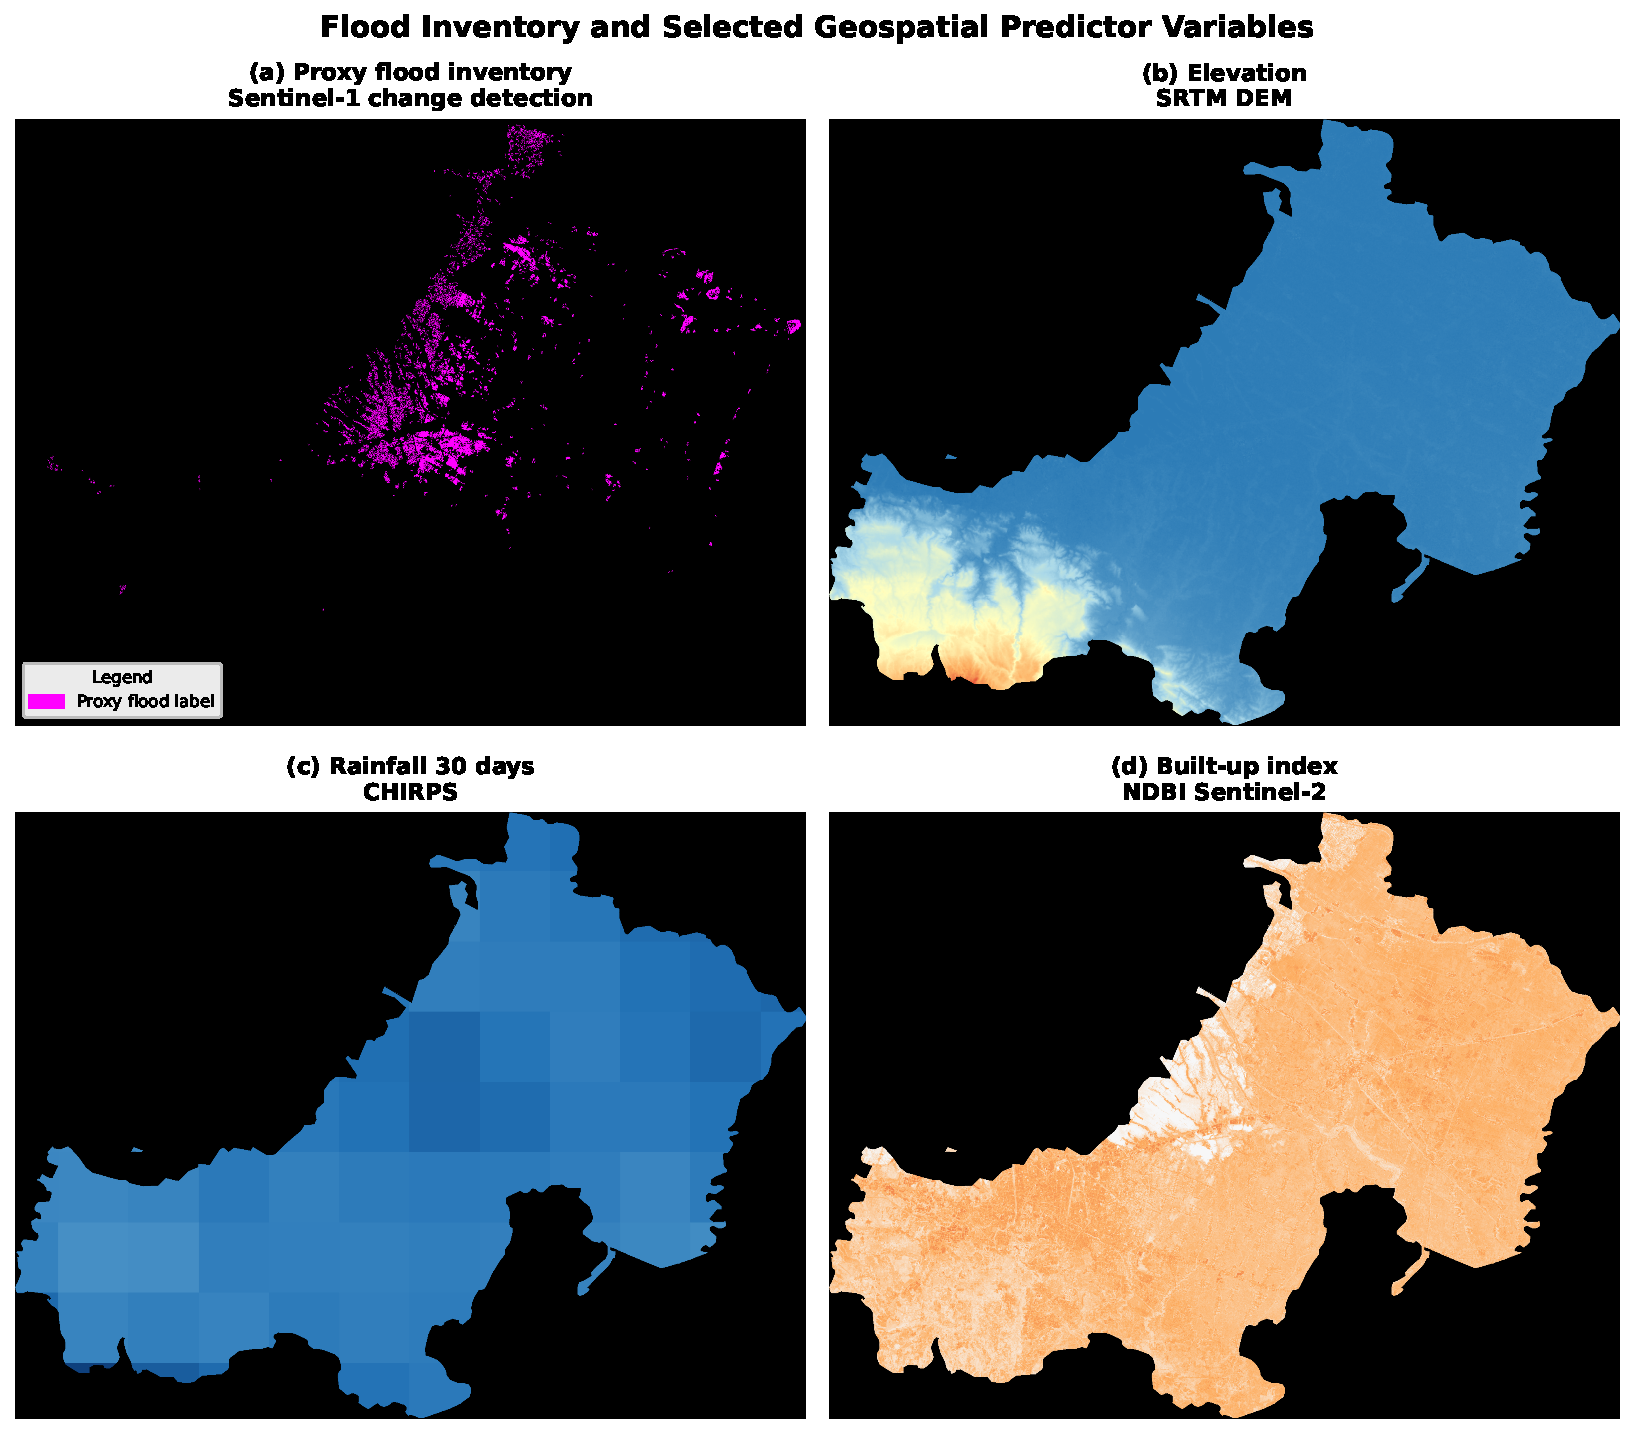
\includegraphics[width=0.55\textwidth]{figures_pdf/image1}
\caption{Sentinel-1-derived flood inventory and selected geospatial predictors.
Source: processed from Google Earth Engine outputs.}
\label{fig:flood-inventory-predictors}
\end{figure}
 
%==================================
\section{Methodology}\label{methods}
 
\subsection{Sentinel-1 Flood Inventory Generation}\label{sentinel-1-flood-inventory-generation}

The target label was constructed from Sentinel-1 GRD VH-backscatter change
detection \cite{unspider2024} for the March 2024 flood event, using a pre-event
composite (25 February -- 12 March 2024) and a post-event composite
(15 -- 31 March 2024). Both composites are per-orbit median composites of all
Interferometric Wide-swath acquisitions covering the study area within each
window. Backscatter values in dB were converted to power scale, and the
pre/post power ratio was computed so that a post-event backscatter drop yields
a ratio greater than one.

A pixel was labelled as flood when \emph{all} of the following conditions
held: (1) the pre/post VH power ratio exceeded 1.25; (2) the post-event VH
backscatter was below $-18$~dB, ensuring a genuinely water-like scattering
regime rather than any small change; (3) the pixel was not permanent water,
defined as a JRC Global Surface Water occurrence of at least 80\%; (4) the SRTM
slope was below $5^{\circ}$, excluding steep surfaces that produce
geometry-induced backscatter drops; and (5) the pixel belonged to a connected
flood cluster of at least eight pixels at the 30~m sampling scale, which
suppresses isolated speckle-induced false detections. Pixels satisfying these
constraints were labelled as flood, while all other sampled pixels were
labelled as non-flood. The combined threshold set represents a compromise
between retaining plausible flood signals and limiting over-detection caused by
water-like surfaces; the sensitivity of the resulting extent to the ratio
threshold is quantified below.
 
A threshold sensitivity analysis showed that estimated flood extent declined
from 56.11 km$^2$ at a ratio threshold of 1.15 to 44.07 km$^2$ at 1.50. This
monotonic reduction indicates that the flood inventory is threshold-sensitive,
as expected in SAR-based flood mapping. The selected threshold therefore
represents a compromise between retaining plausible flood signals and limiting
over-detection caused by water-like surfaces.
 
\subsection{Sampling Strategy and Class Imbalance Handling}\label{sampling-strategy-and-class-imbalance-handling}
 
The raw stratified sample contained 3,935 observations, consisting of 3,000
non-flood and 935 flood samples. This imbalance emerged because the
Semarang-Demak-only region contains fewer flood-labelled pixels than the
surrounding-region ROI. Directly training and evaluating models on this
imbalance could bias predictions toward the non-flood class and inflate accuracy
while weakening flood recall.
 
To reduce majority-class dominance, the final modelling dataset was balanced
through undersampling the non-flood class, resulting in 1,870 observations with
935 non-flood and 935 flood samples. This decision improves class comparability
and makes recall, precision, and F1-score more meaningful for flood detection.
However, it also reduces the diversity of non-flood samples. Therefore, the
balanced dataset is interpreted as a modelling design for fair classification
rather than a representation of natural flood prevalence in the landscape.
 
\begin{table}[ht]
\centering
\caption{Class distribution before and after imbalance handling.}
\label{tab:class-distribution}
\begin{tabular}{>{\raggedright}p{2.8cm}
                c c c
                >{\raggedright\arraybackslash}p{5.5cm}}
\hline
\textbf{Dataset} & \textbf{Non-flood} & \textbf{Flood} & \textbf{Total} &
\textbf{Purpose} \\
\hline
Raw sample & 3000 & 935 & 3935 & Preserves available sample distribution but is
imbalanced \\
Balanced sample & 935 & 935 & 1870 & Used for final model comparison and SHAP
interpretation \\
\hline
\end{tabular}
\end{table}
 
\subsection{Ensemble Learning Models and Evaluation}\label{ensemble-learning-models-and-evaluation}

Seven ensemble models were evaluated: Random Forest \cite{breiman2001},
Extra Trees, Gradient Boosting, XGBoost \cite{chen2016}, LightGBM \cite{ke2017},
CatBoost \cite{prokhorenkova2018}, and a stacking ensemble. Tree-based
ensemble models were selected because flood susceptibility is expected to involve
non-linear and threshold-like relationships between variables, such as abrupt
increases in susceptibility near water bodies, low elevation, or high rainfall
accumulation.

Table \ref{tab:hyperparameters} reports the hyperparameter configuration of
each model. The configuration follows common defaults for tabular
geospatial classification with moderate depth regularization, and all models
were trained with a fixed random seed (42) for reproducibility. The stacking
ensemble combines Random Forest, Extra Trees, XGBoost, and LightGBM as base
learners with a class-weighted logistic regression meta-learner using five-fold
internal cross-validation. The optimized classification threshold for every
model was determined using the Youden index from its ROC curve.

\begin{table}[ht]
\centering
\caption{Hyperparameter settings of the seven ensemble models (random seed = 42 for all models).}
\label{tab:hyperparameters}
\begin{tabular}{>{\raggedright}p{3.4cm} >{\raggedright\arraybackslash}p{10.2cm}}
\hline
\textbf{Model} & \textbf{Hyperparameters} \\
\hline
Random Forest & 400 trees; \texttt{min\_samples\_leaf} = 2; class weight = balanced \\
Extra Trees & 400 trees; \texttt{min\_samples\_leaf} = 2; class weight = balanced \\
Gradient Boosting & 250 stages; learning rate = 0.04; max depth = 3 \\
XGBoost & 350 rounds; learning rate = 0.04; max depth = 4; subsample = 0.85; column sample = 0.85; eval metric = logloss \\
LightGBM & 350 rounds; learning rate = 0.04; 31 leaves; subsample = 0.85; column sample = 0.85; class weight = balanced \\
CatBoost & 350 iterations; learning rate = 0.04; depth = 5; loss = Logloss; eval metric = AUC \\
Stacking ensemble & Base: Random Forest + Extra Trees + XGBoost + LightGBM; meta-learner: logistic regression (max iter = 2000, class weight = balanced); internal 5-fold CV \\
\hline
\end{tabular}
\end{table}

Model performance was evaluated using ROC-AUC, accuracy, precision, recall, and
F1-score. In susceptibility mapping, recall is particularly important because
false negatives may omit vulnerable zones. Nevertheless, precision is also
relevant because excessive false positives may overstate areas requiring
intervention. F1-score therefore provides a useful balance between omission and
commission errors.

\subsection{Data Splitting, Evaluation Protocol, and SHAP Data}\label{data-splitting-protocol}

The 1,870 balanced samples were divided once into a training set (75\%; 1,402
samples) and an independent held-out test set (25\%; 468 samples) using a
stratified random split with a fixed seed. All seven models were trained
exclusively on the training set, and all headline performance figures in
Table \ref{tab:model-performance} were computed on the held-out test set, which
was not used in any stage of model fitting or tuning. Because the split is
random rather than spatial, neighbouring pixels with highly similar
environmental conditions can appear on both sides of the split; the spatial
block cross-validation in Section \ref{spatial-cv-results} quantifies the
effect of this design on generalization estimates. The SHAP analysis of the
best model was computed on a random subsample of 1,000 rows drawn from the
training set only, so no information from the held-out test set enters either
the interpretation or the reported explanation values. The original training
run was executed on Google Colab. For the additional analyses reported in this
revised version (statistical model comparison, spatial block cross-validation,
correlation diagnostics, and the SHAP dependence analysis), the full pipeline
was re-run with the same fixed seed in two environments: a Kaggle environment
(Python 3.12.13, scikit-learn 1.6.1, XGBoost 3.2.0, LightGBM 4.6.0, CatBoost
1.2.10, SHAP 0.51.0, NumPy 2.0.2, pandas 2.3.3) whose held-out test predictions
reproduce six of the seven AUCs of Table \ref{tab:model-performance} to six
decimal places (the stacking ensemble differs by 0.002), and a local
environment (Python 3.14.6, scikit-learn 1.9.0, XGBoost 3.4.1, LightGBM 4.7.0,
CatBoost 1.2.10, SHAP 0.52.0, NumPy 2.5.2, pandas 3.0.5, SciPy 1.18.1). The
statistical model comparison was computed on the predictions that reproduce
Table \ref{tab:model-performance} exactly, and all robustness diagnostics agree
between the two environments within 0.006 ROC-AUC.

\subsection{Statistical Comparison of Model Performance}\label{statistical-comparison}

Because the leading models differ by small ROC-AUC margins, pairwise
differences against Random Forest were assessed with two complementary tests
computed on the same held-out test predictions: DeLong's test for correlated
ROC curves \cite{delong1988} and a paired bootstrap procedure with 10,000 resamples of the test
set, reporting 95\% confidence intervals of the AUC difference. Both tests
evaluate whether the observed ranking reflects a systematic advantage or
sampling variability.

\subsection{Spatial Block Cross-Validation}\label{spatial-cv-protocol}

To assess spatial generalization independently of the random split, all models
were additionally evaluated with a five-fold spatial block cross-validation
design. The study area was partitioned into approximately $10 \times 10$~km
blocks ($0.1^{\circ}$ grid cells) defined from the geographic coordinates of
each sample, and entire blocks were assigned to folds so that no block
contributes samples to both training and evaluation within a fold. This design
prevents the leakage of spatially autocorrelated information between
neighbouring pixels across the train--test boundary and therefore provides a
more conservative estimate of map generalization to unsampled areas.
 
\subsection{SHAP Interpretation}\label{shap-interpretation}

SHAP was applied to the best-performing model to quantify the contribution of
each predictor to model output. The interpretation was computed on a random
subsample of 1,000 rows drawn from the training set only; the held-out test set
played no role in the explanation. For binary classification, the SHAP values
were
interpreted for the flood class. This is methodologically important because
using the raw multi-class SHAP array without selecting the positive class can
produce misleading interaction-style plots. The corrected SHAP workflow therefore
allows the analysis to infer not only which variables are important, but also
how hydrological, rainfall, vegetation, and built-up factors shape the predicted
flood susceptibility signal.
 
%==================================
\section{Empirical Results}\label{results}
 
\subsection{Model Performance}\label{model-performance}

\begin{table}[ht]
\centering
\caption{Optimized model performance on the balanced dataset. Test-set metrics
were computed on the 25\% held-out split. CV AUC columns report mean $\pm$ SD
over five-fold cross-validation with random stratified folds and with spatial
block folds ($\sim$10 km blocks), respectively.}
\label{tab:model-performance}
\begin{tabular}{lccccc cc}
\hline
\textbf{Model} & \textbf{ROC-AUC} & \textbf{Accuracy} & \textbf{Precision} &
\textbf{Recall} & \textbf{F1-score} & \textbf{CV AUC (random)} & \textbf{CV AUC (spatial)} \\
\hline
RandomForest      & 0.852 & 0.791 & 0.727 & 0.932 & 0.816 & $0.842 \pm 0.019$ & $0.593 \pm 0.094$ \\
StackingEnsemble  & 0.850 & 0.786 & 0.743 & 0.876 & 0.804 & $0.841 \pm 0.018$ & $0.603 \pm 0.094$ \\
CatBoost          & 0.849 & 0.786 & 0.743 & 0.876 & 0.804 & $0.835 \pm 0.018$ & $0.565 \pm 0.079$ \\
XGBoost           & 0.842 & 0.778 & 0.720 & 0.910 & 0.804 & $0.825 \pm 0.017$ & $0.602 \pm 0.081$ \\
LightGBM          & 0.836 & 0.782 & 0.734 & 0.885 & 0.802 & $0.824 \pm 0.021$ & $0.614 \pm 0.089$ \\
ExtraTrees        & 0.835 & 0.778 & 0.766 & 0.799 & 0.782 & $0.831 \pm 0.020$ & $0.591 \pm 0.082$ \\
GradientBoosting  & 0.831 & 0.767 & 0.736 & 0.833 & 0.782 & $0.816 \pm 0.021$ & $0.598 \pm 0.072$ \\
\hline
\end{tabular}
\end{table}
 
Random Forest produced the highest ROC-AUC (0.852) and the best F1-score (0.816)
at the optimized threshold, with accuracy = 0.791, precision = 0.727, and recall
= 0.932. This result indicates that Random Forest offered the strongest balance
between discrimination and flood-class sensitivity in the balanced
Semarang-Demak dataset.
 
The margin between Random Forest, Stacking Ensemble, CatBoost, XGBoost, and
LightGBM was not large. This suggests that the predictive signal is not unique
to a single algorithm, but is consistently learnable by several tree-based
ensembles. Such convergence strengthens the credibility of the geospatial
predictor set: if only one algorithm performed well while the others failed, the
result might indicate model-specific instability. Instead, the relatively close
performance implies that the dataset contains a coherent flood-susceptibility
structure.
 
The optimized Random Forest threshold was lower than 0.50, which is expected in
a susceptibility problem where flood omission is costlier than moderate
overprediction. The model prioritizes recall, meaning that more flood-prone
samples are captured even at the expense of additional false positives. In
risk-screening applications, this is generally preferable because areas falsely
flagged as susceptible can be refined through field validation, while missed
flood-prone areas may remain unmanaged.
 
\begin{figure}[htbp]
\centering
\begin{subfigure}{0.55\textwidth}
\centering
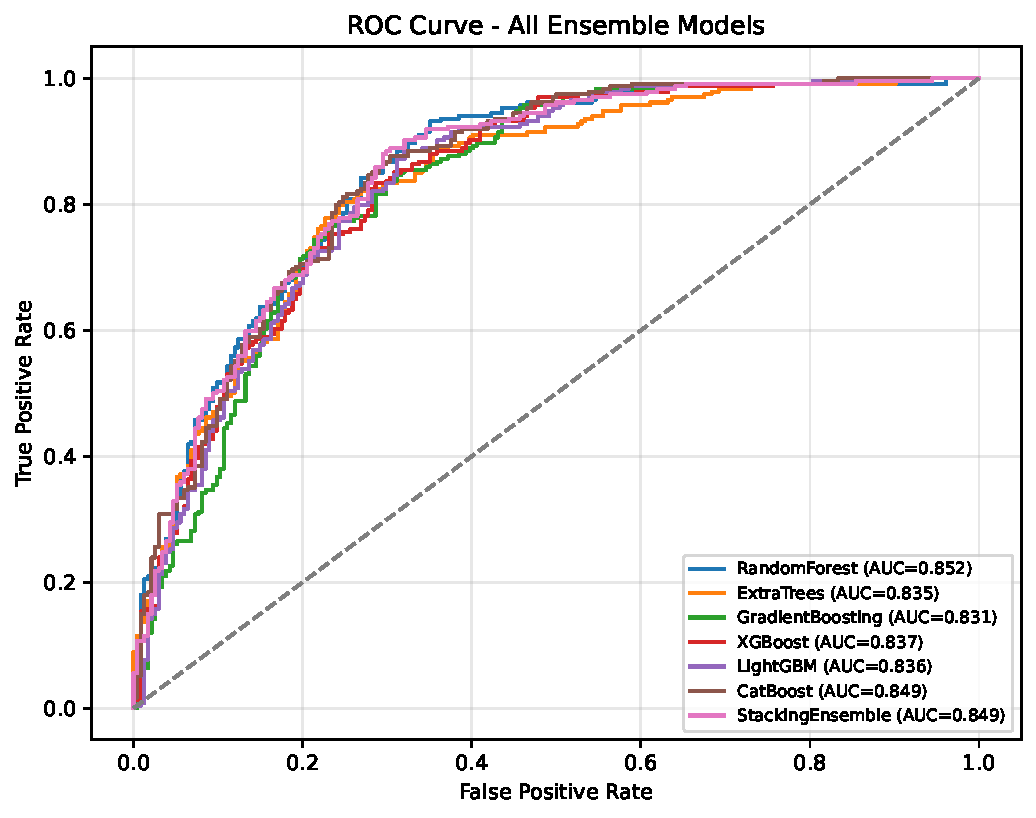
\includegraphics[width=\textwidth]{figures_pdf/image2}
\caption{ROC curve.}
\end{subfigure}
 
\vspace{0.5em}
\begin{subfigure}{0.55\textwidth}
\centering
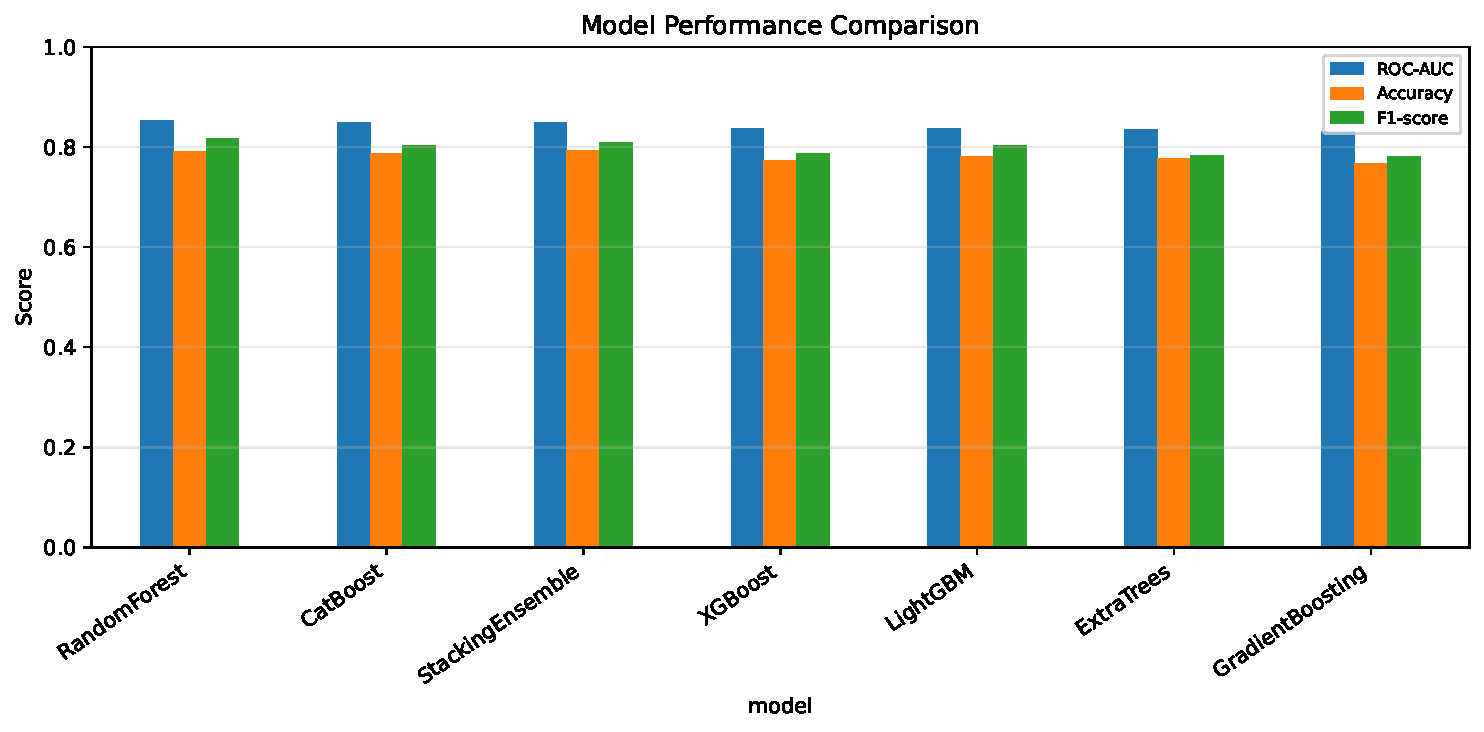
\includegraphics[width=\textwidth]{figures_pdf/image3}
\caption{Model performance summary.}
\end{subfigure}
\caption{ROC curve and model performance summary. Source: model evaluation
outputs.}
\label{fig:model-performance}
\end{figure}
 
\subsection{Error Structure from Confusion Matrices}\label{error-structure-from-confusion-matrices}

\begin{figure}[htbp]
\centering
\begin{subfigure}{1\textwidth}
\centering
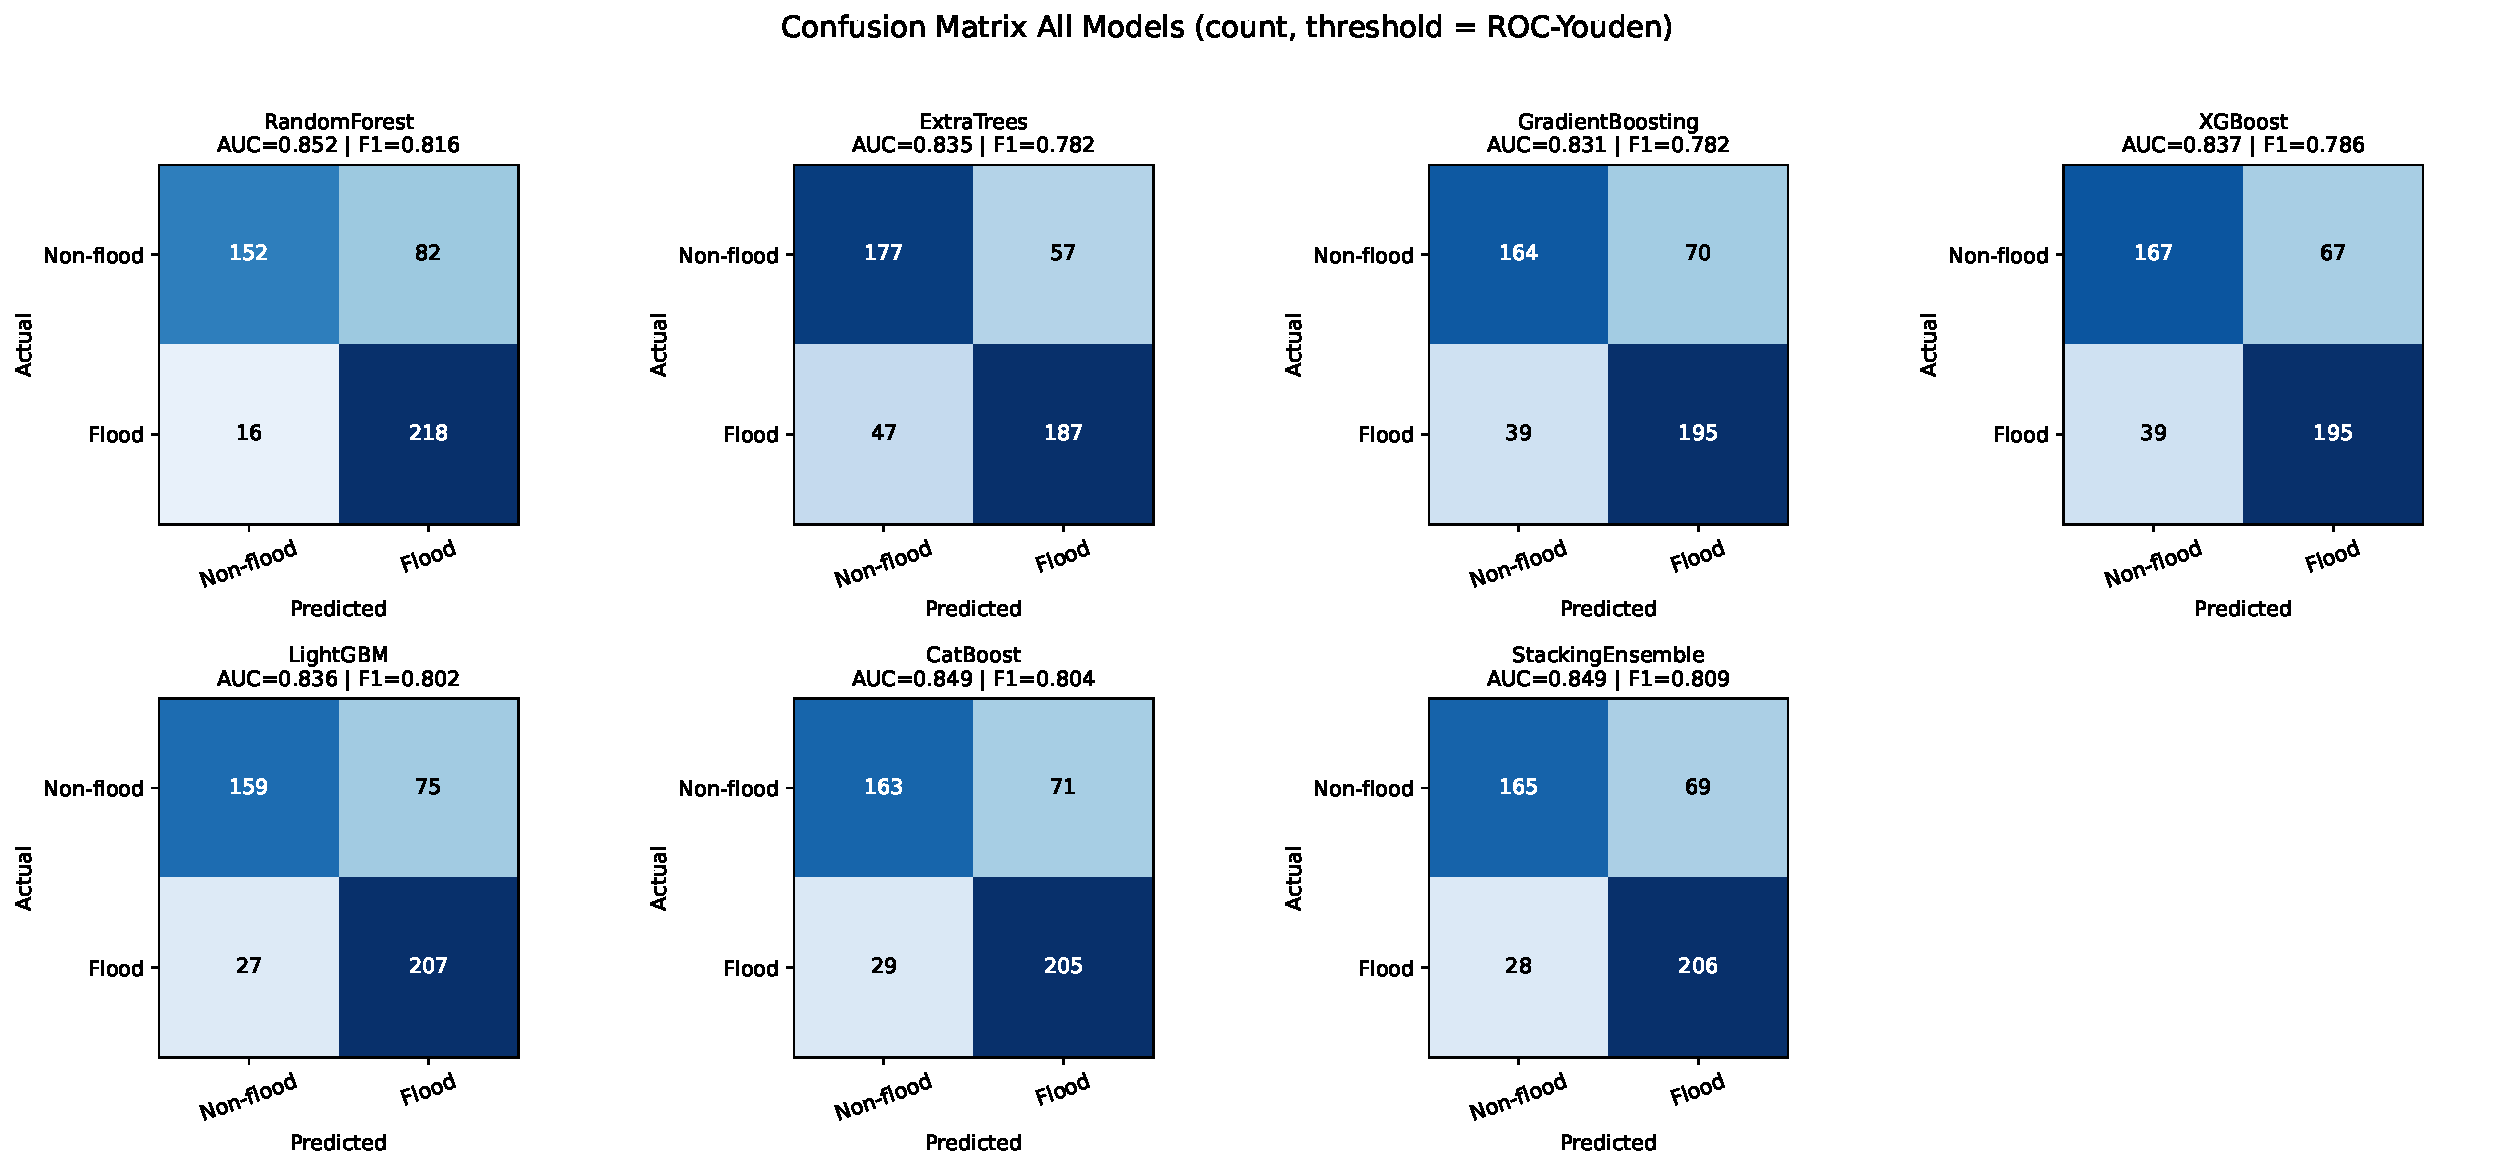
\includegraphics[width=\textwidth]{figures_pdf/image4}
\caption{Confusion matrix counts.}
\end{subfigure}
 
\vspace{0.5em}
\begin{subfigure}{1\textwidth}
\centering
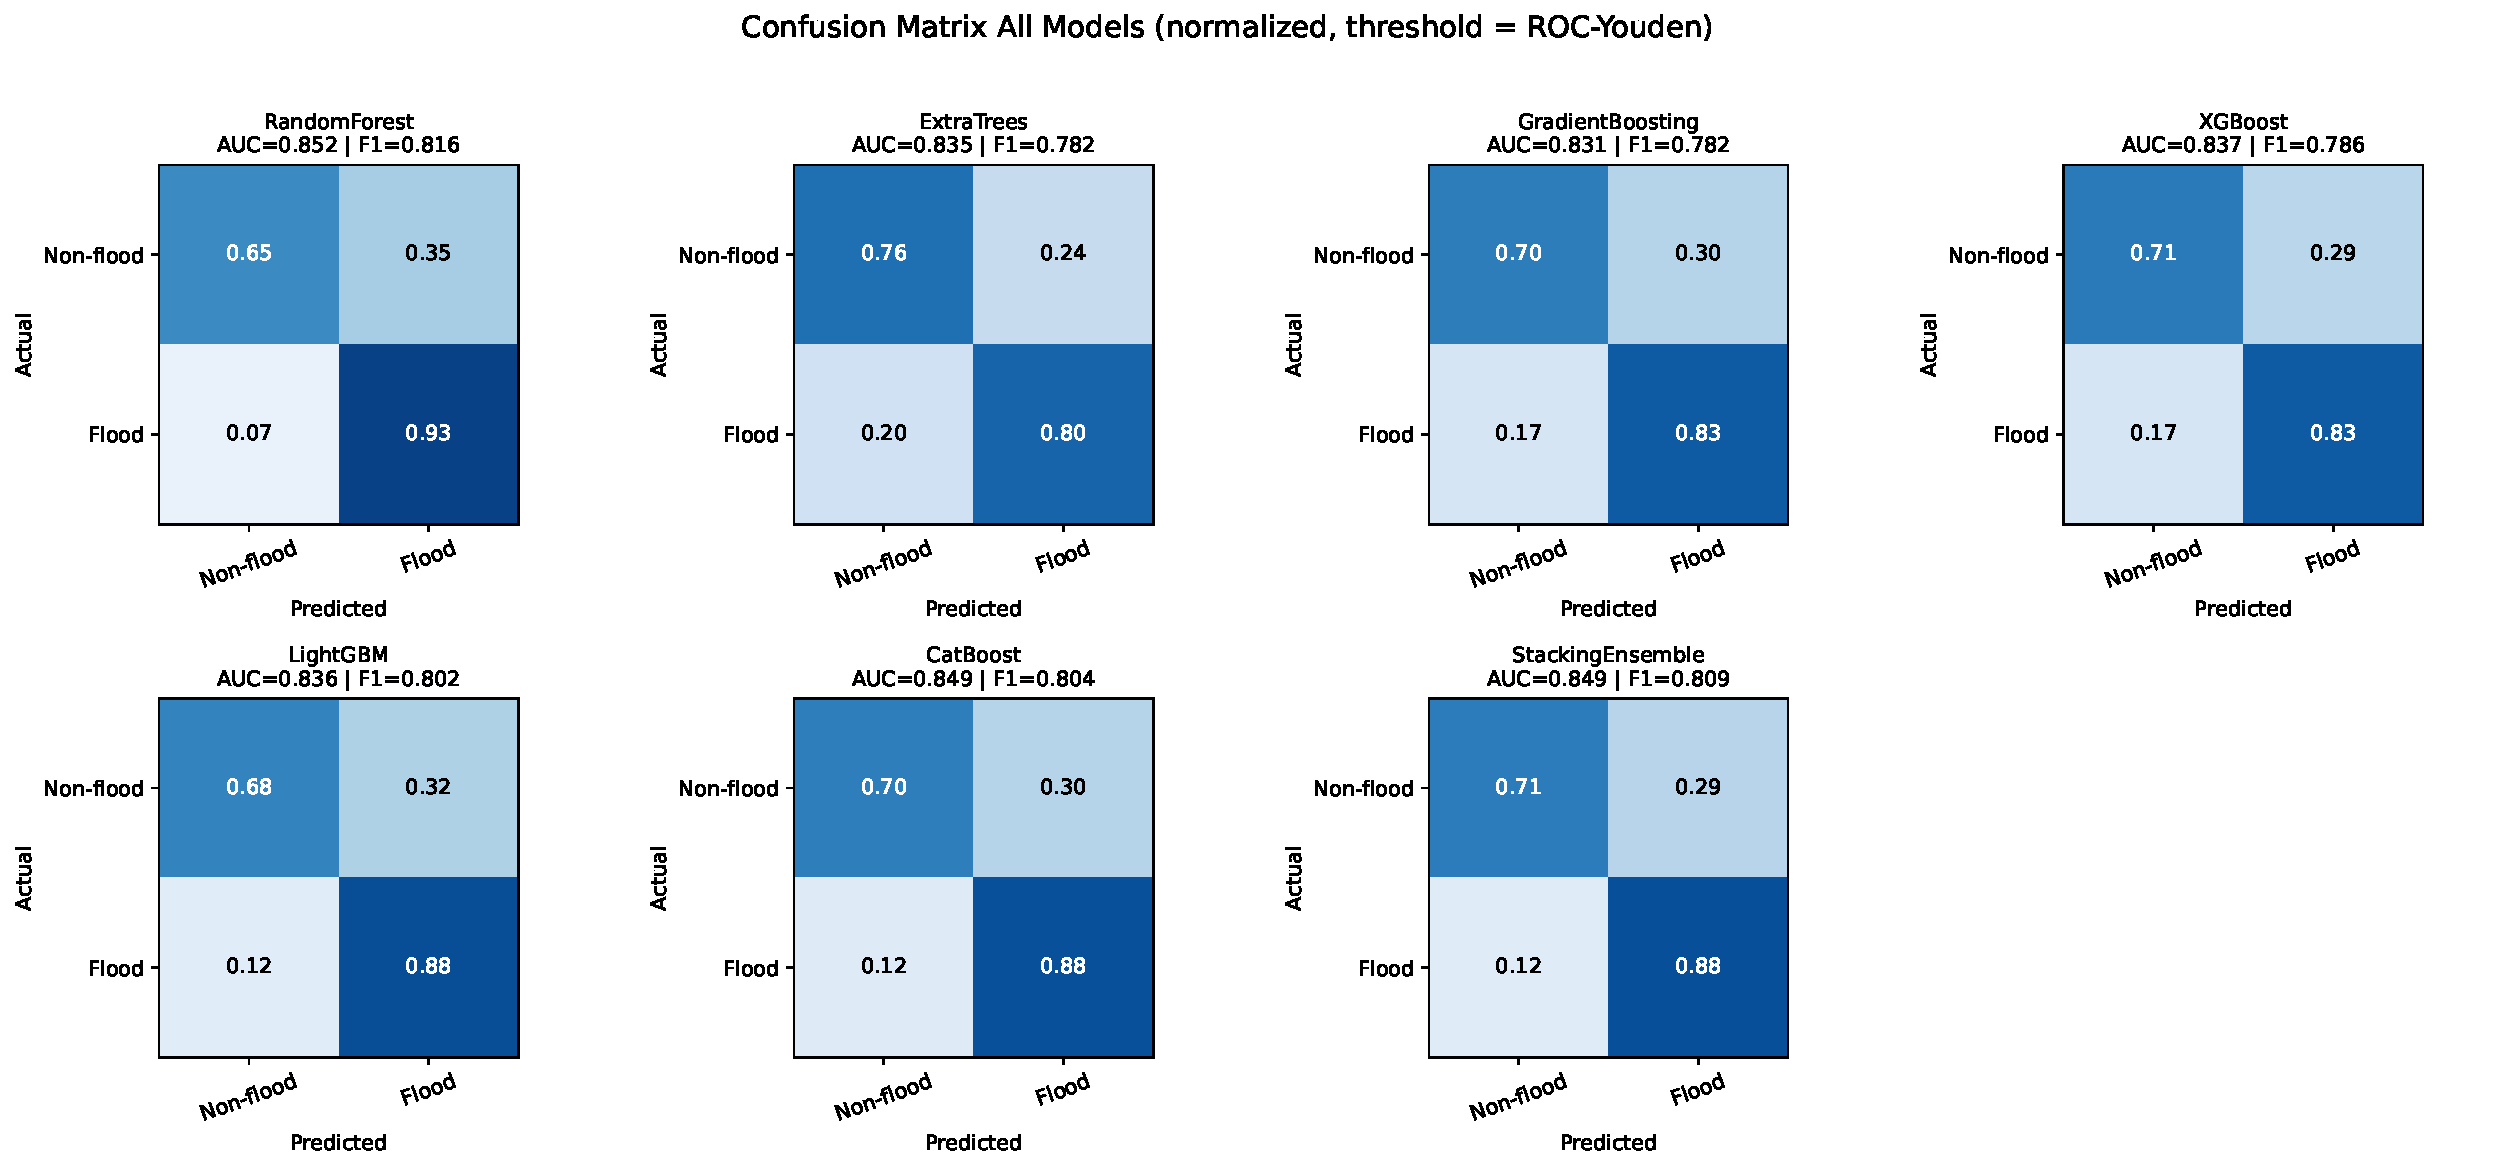
\includegraphics[width=\textwidth]{figures_pdf/image5}
\caption{Normalized confusion matrices.}
\end{subfigure}
\caption{Confusion matrices for all evaluated models. Source: model evaluation
outputs. The normalized matrix shows class-wise error proportions.}
\label{fig:confusion-matrices}
\end{figure}
 
The confusion matrices show that model evaluation should not be reduced to
overall accuracy. In flood susceptibility mapping, false negatives and false
positives have asymmetric implications. False negatives indicate locations
labelled as flood but predicted as non-flood, which may underestimate flood-prone
areas. False positives indicate locations predicted as susceptible but labelled
as non-flood; these may not always be purely erroneous because susceptibility
refers to similarity with flood-prone conditions, not necessarily inundation
during the selected event.
 
The high recall of Random Forest indicates that the model is conservative in
capturing flood-prone samples. This behaviour is suitable for preliminary
susceptibility screening, especially in coastal urban planning where
underestimating potential hazard zones can be more consequential than flagging
extra areas for further inspection. However, this also means that the resulting
susceptibility map should be validated before being used for site-specific
engineering decisions.

\subsection{Statistical Model Comparison and Spatially Validated Performance}\label{spatial-cv-results}

The DeLong tests and paired bootstrap comparisons on the held-out test
predictions show that Random Forest is statistically indistinguishable from the
other leading models. The differences against the stacking ensemble
($\Delta$AUC $= 0.002$, $p = 0.652$), CatBoost ($\Delta$AUC $= 0.003$,
$p = 0.691$), XGBoost ($\Delta$AUC $= 0.010$, $p = 0.174$), and LightGBM
($\Delta$AUC $= 0.016$, $p = 0.072$) are all non-significant, and the 95\%
bootstrap confidence intervals of these differences all include zero (for
example, $[-0.002, +0.033]$ against LightGBM). Only the comparisons against the
two lowest-ranked models reach marginal significance: Extra Trees
($\Delta$AUC $= 0.018$, $p = 0.034$) and Gradient Boosting ($\Delta$AUC
$= 0.022$, $p = 0.040$). Random Forest should accordingly be read as the model
with the highest point estimate, statistically inseparable from the rest of the
leading cluster under this configuration, with a small but detectable margin
over the two weakest models.

The spatial block cross-validation results provide an important corrective
perspective on the headline metrics. When entire $\sim$10 km blocks are held
out, the five-fold cross-validated ROC-AUC of all models drops to the
0.56--0.61 range (Table \ref{tab:model-performance}, last column), compared with
0.82--0.84 under random stratified folds. This gap confirms that the random
split benefits from spatial autocorrelation between neighbouring training and
test pixels, and that the held-out estimates of Table \ref{tab:model-performance}
are optimistic with respect to generalization to geographically distinct areas.
Three implications follow. First, the model ranking is stable across both
validation designs, so the comparative conclusion is not an artefact of the
splitting strategy. Second, the susceptibility map should be interpreted as an
interpolation within the environmental and spatial domain represented by the
training samples rather than a transferable predictor for other regions. Third,
the persistent water-proximity signal that dominates the SHAP analysis partly
reflects local spatial context, which reinforces the cautious interpretation of
Section \ref{dominant-role-water-rainfall}.

\subsection{Feature Importance and SHAP Explanation}\label{feature-importance-and-shap-explanation}

\begin{table}[ht]
\centering
\caption{Top SHAP-based predictor contributions for the flood class.}
\label{tab:shap-contributions}
\begin{tabular}{lc}
\hline
\textbf{Predictor} & \textbf{Mean $|\text{SHAP}|$} \\
\hline
dist\_perm\_water & 0.058 \\
rain\_30d         & 0.042 \\
ndvi              & 0.036 \\
rain\_7d          & 0.031 \\
upa\_log          & 0.030 \\
mndwi             & 0.026 \\
ndbi              & 0.025 \\
river\_width      & 0.024 \\
dist\_river       & 0.024 \\
ndwi              & 0.023 \\
slope             & 0.020 \\
elevation         & 0.013 \\
\hline
\end{tabular}
\end{table}
 
\begin{figure}[htbp]
\centering
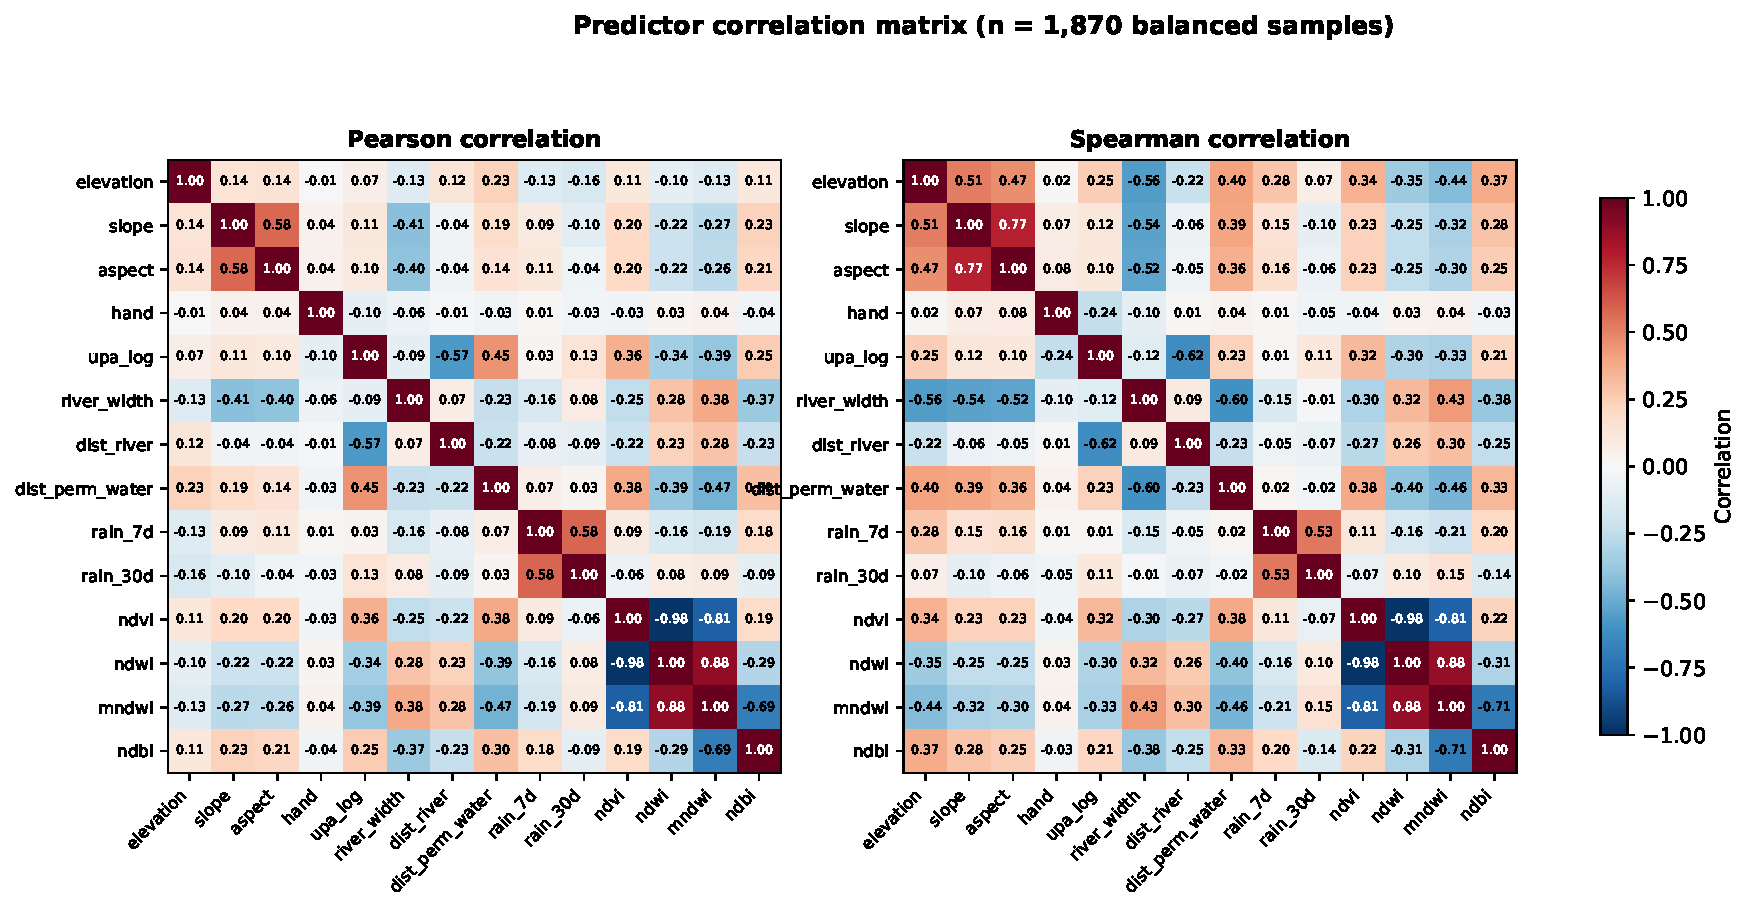
\includegraphics[width=0.95\textwidth]{figures_pdf/image11}
\caption{Pearson and Spearman correlation matrices of the continuous
predictors ($n = 1{,}870$). The four Sentinel-2 spectral indices form a highly
collinear block, as expected from their shared input bands.}
\label{fig:correlation-matrix}
\end{figure}

Because NDVI, NDWI, MNDWI, and NDBI are derived from overlapping Sentinel-2
bands, their pairwise Pearson correlations were inspected
(Figure \ref{fig:correlation-matrix}). The indices are indeed strongly
collinear: NDVI and NDWI correlate at $r = -0.98$, NDWI and MNDWI at $r = 0.88$,
and MNDWI and NDBI at $r = -0.69$, whereas NDBI and NDVI are only weakly
correlated ($r = 0.19$). This collinearity is inconsequential for the predictive
models, because tree-based ensembles are insensitive to linear dependence among
predictors and the goal is discrimination rather than coefficient estimation.
For the SHAP ranking, however, it implies that importance is shared among
correlated indices and that individual ranks within the spectral-index block
should not be over-interpreted; the aggregated signal of the index block is
meaningful, but the ordering of, for example, MNDWI versus NDWI is not
identifiable. The remaining non-spectral predictors are only moderately
correlated (maximum $|r| = 0.58$, between 7-day and 30-day antecedent
rainfall), so their SHAP ranks are more directly interpretable.

\begin{figure}[htbp]
\centering
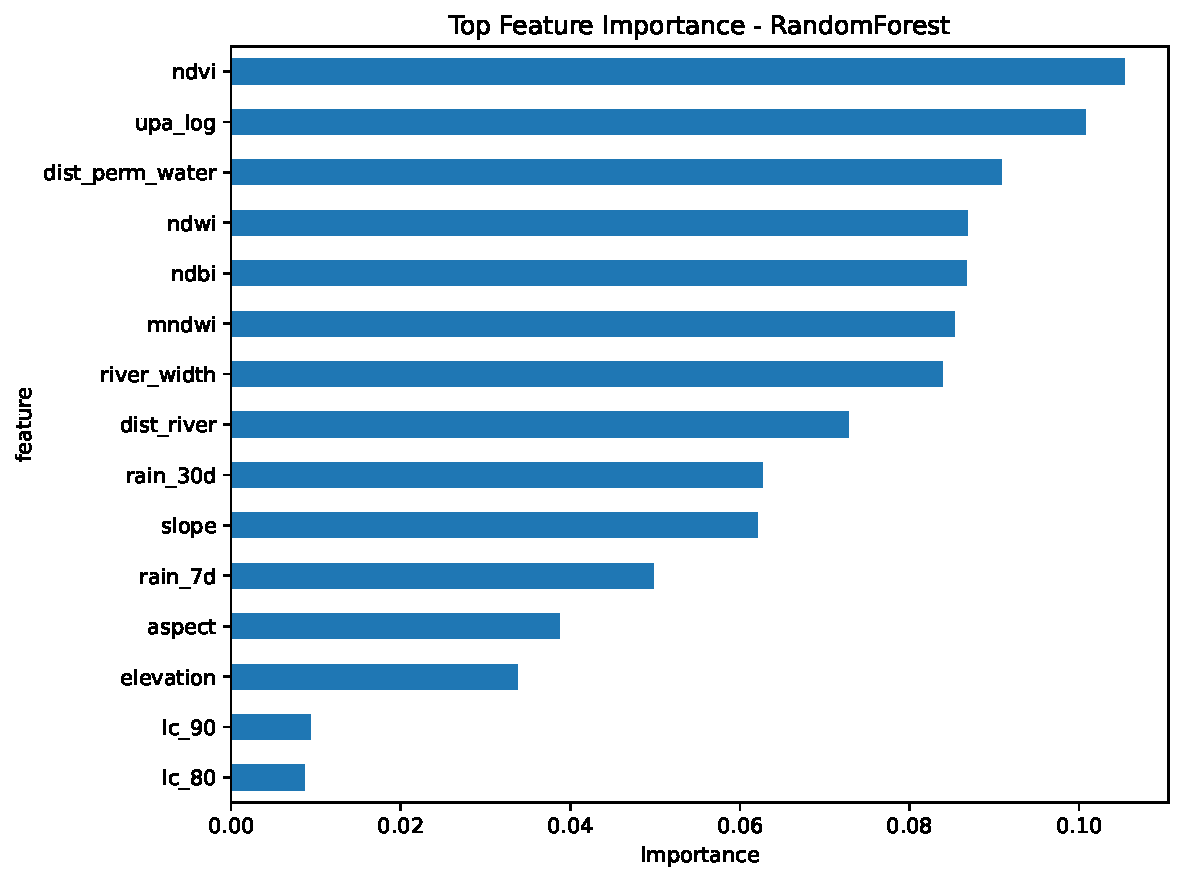
\includegraphics[width=0.55\textwidth]{figures_pdf/image6}
\caption{Random Forest feature importance. Source: Python model interpretation
outputs.}
\label{fig:feature-importance}
\end{figure}
 
\begin{figure}[htbp]
\centering

\begin{subfigure}[t]{0.45\textwidth}
    \centering
    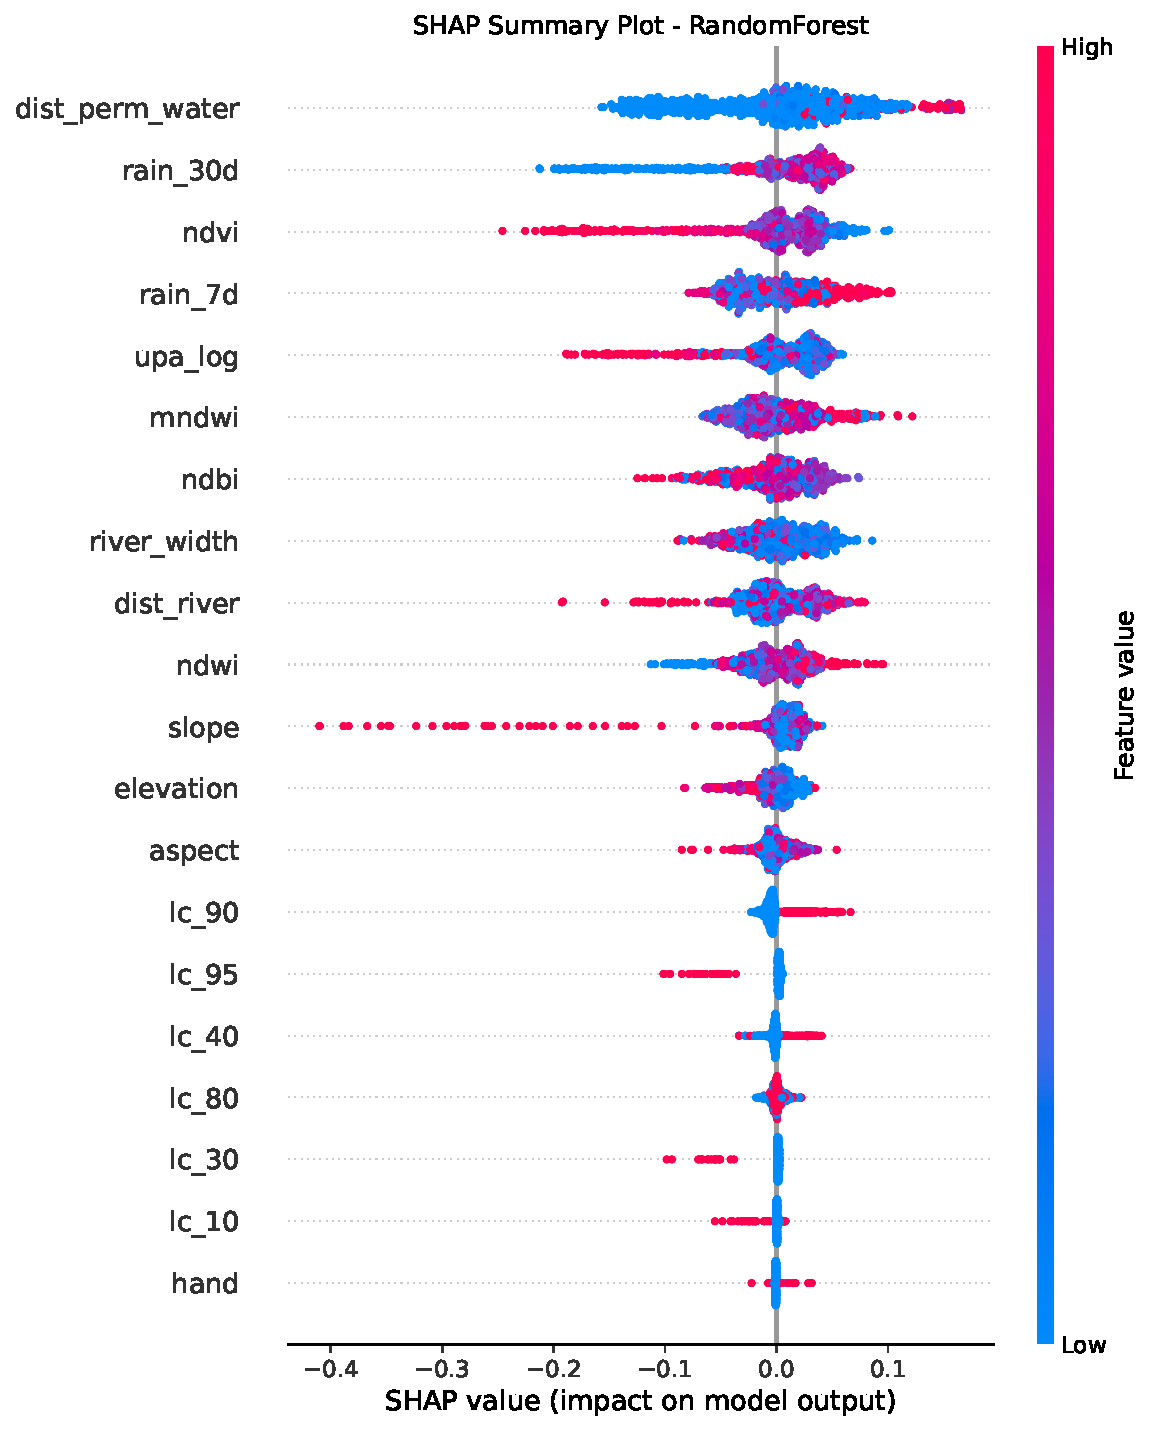
\includegraphics[width=\linewidth]{figures_pdf/image7}
    \caption{SHAP summary plot for the positive flood class.}
    \label{fig:shap-summary}
\end{subfigure}
\hfill
\begin{subfigure}[t]{0.45\textwidth}
    \centering
    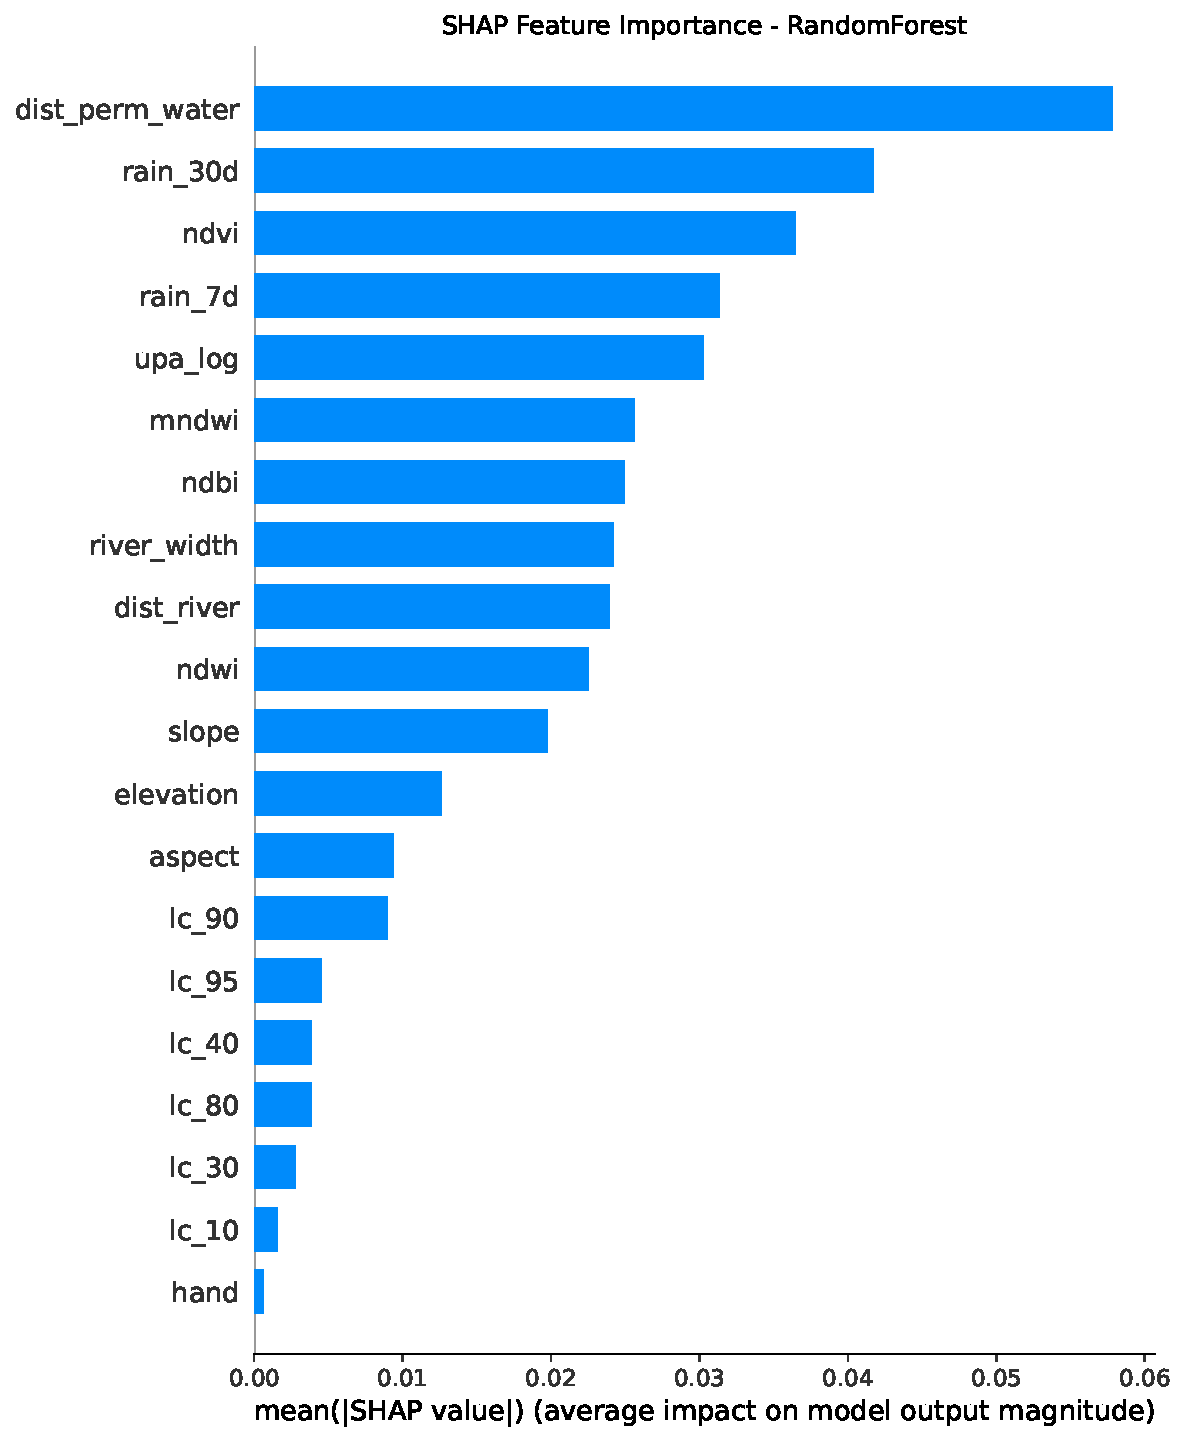
\includegraphics[width=\linewidth]{figures_pdf/image8}
    \caption{SHAP-based predictor contribution ranking for the flood class.}
    \label{fig:shap-bar}
\end{subfigure}

\caption{SHAP-based interpretation of the flood classification model.}
\label{fig:shap-interpretation}
\end{figure}
 
The Random Forest feature importance and SHAP results jointly indicate that
flood susceptibility in the Semarang-Demak coastal area is governed by
interacting hydrological proximity, rainfall forcing, vegetation condition, and
built-up intensity. Random Forest impurity-based importance ranked NDVI,
upstream drainage area, distance to permanent water, NDWI, NDBI, MNDWI, river
width, distance to river, rainfall, and slope among the key variables. The SHAP
ranking refined this interpretation by identifying distance to permanent water,
30-day rainfall, NDVI, 7-day rainfall, upstream drainage area, MNDWI, NDBI,
river width, distance to river, and NDWI as the strongest contributors to
prediction.
 
The dominance of distance to permanent water is physically plausible. In a
coastal lowland, locations near permanent water bodies, rivers, ponds, drainage
channels, and wet surfaces often share hydrological connectivity with flood
pathways. The importance of antecedent rainfall reflects the role of accumulated
precipitation in increasing runoff potential, saturating surfaces, and loading
drainage systems. The presence of both 7-day and 30-day rainfall among the
influential predictors suggests that the model captures both short-term event
forcing and antecedent wetness conditions.
 
Vegetation and water indices provide additional surface-state information. NDVI
separates vegetated or agricultural areas from built-up and bare surfaces, and
its SHAP contribution is directionally consistent with susceptibility being
higher in low-vegetation, moisture-laden, or disturbed zones. NDWI and MNDWI
capture open-water and moisture signals, with higher index values producing
positive SHAP contributions that push predictions toward the flood class. NDBI
reflects built-up intensity; its positive mean $|\text{SHAP}|$ implies that
denser urban surfaces, where imperviousness limits infiltration, are associated
with higher model-predicted susceptibility.

Hydrological variables such as upstream drainage area, river width, and distance
to river reinforce the water-proximity argument at the channel scale. Locations
with larger upstream contributing areas or narrower separation from river
channels consistently produce positive SHAP values, consistent with the physical
expectation that drainage convergence amplifies inundation potential. These
variables should be interpreted as derived predictors from global hydrological
datasets rather than field-surveyed drainage infrastructure; their contribution
nevertheless supports the expectation that susceptibility is higher where terrain
and drainage structures concentrate water.

Notably, \texttt{elevation} and \texttt{slope} rank last in SHAP contribution,
with mean $|\text{SHAP}|$ values of 0.013 and 0.020 respectively. In
mountainous or hilly study areas, these variables typically dominate flood
susceptibility models because terrain controls runoff pathways directly. Their
low rank here is an informative finding for a coastal lowland: when topographic
relief is minimal and confined within a narrow elevation range, the
discriminating signal shifts from terrain structure to water proximity and
rainfall accumulation. The SHAP rankings therefore reflect the physical
character of the Semarang-Demak setting rather than a deficiency of the
predictor set.
 
\subsection{Spatial Susceptibility Pattern}\label{spatial-susceptibility-pattern}

\begin{figure}[htbp]
\centering
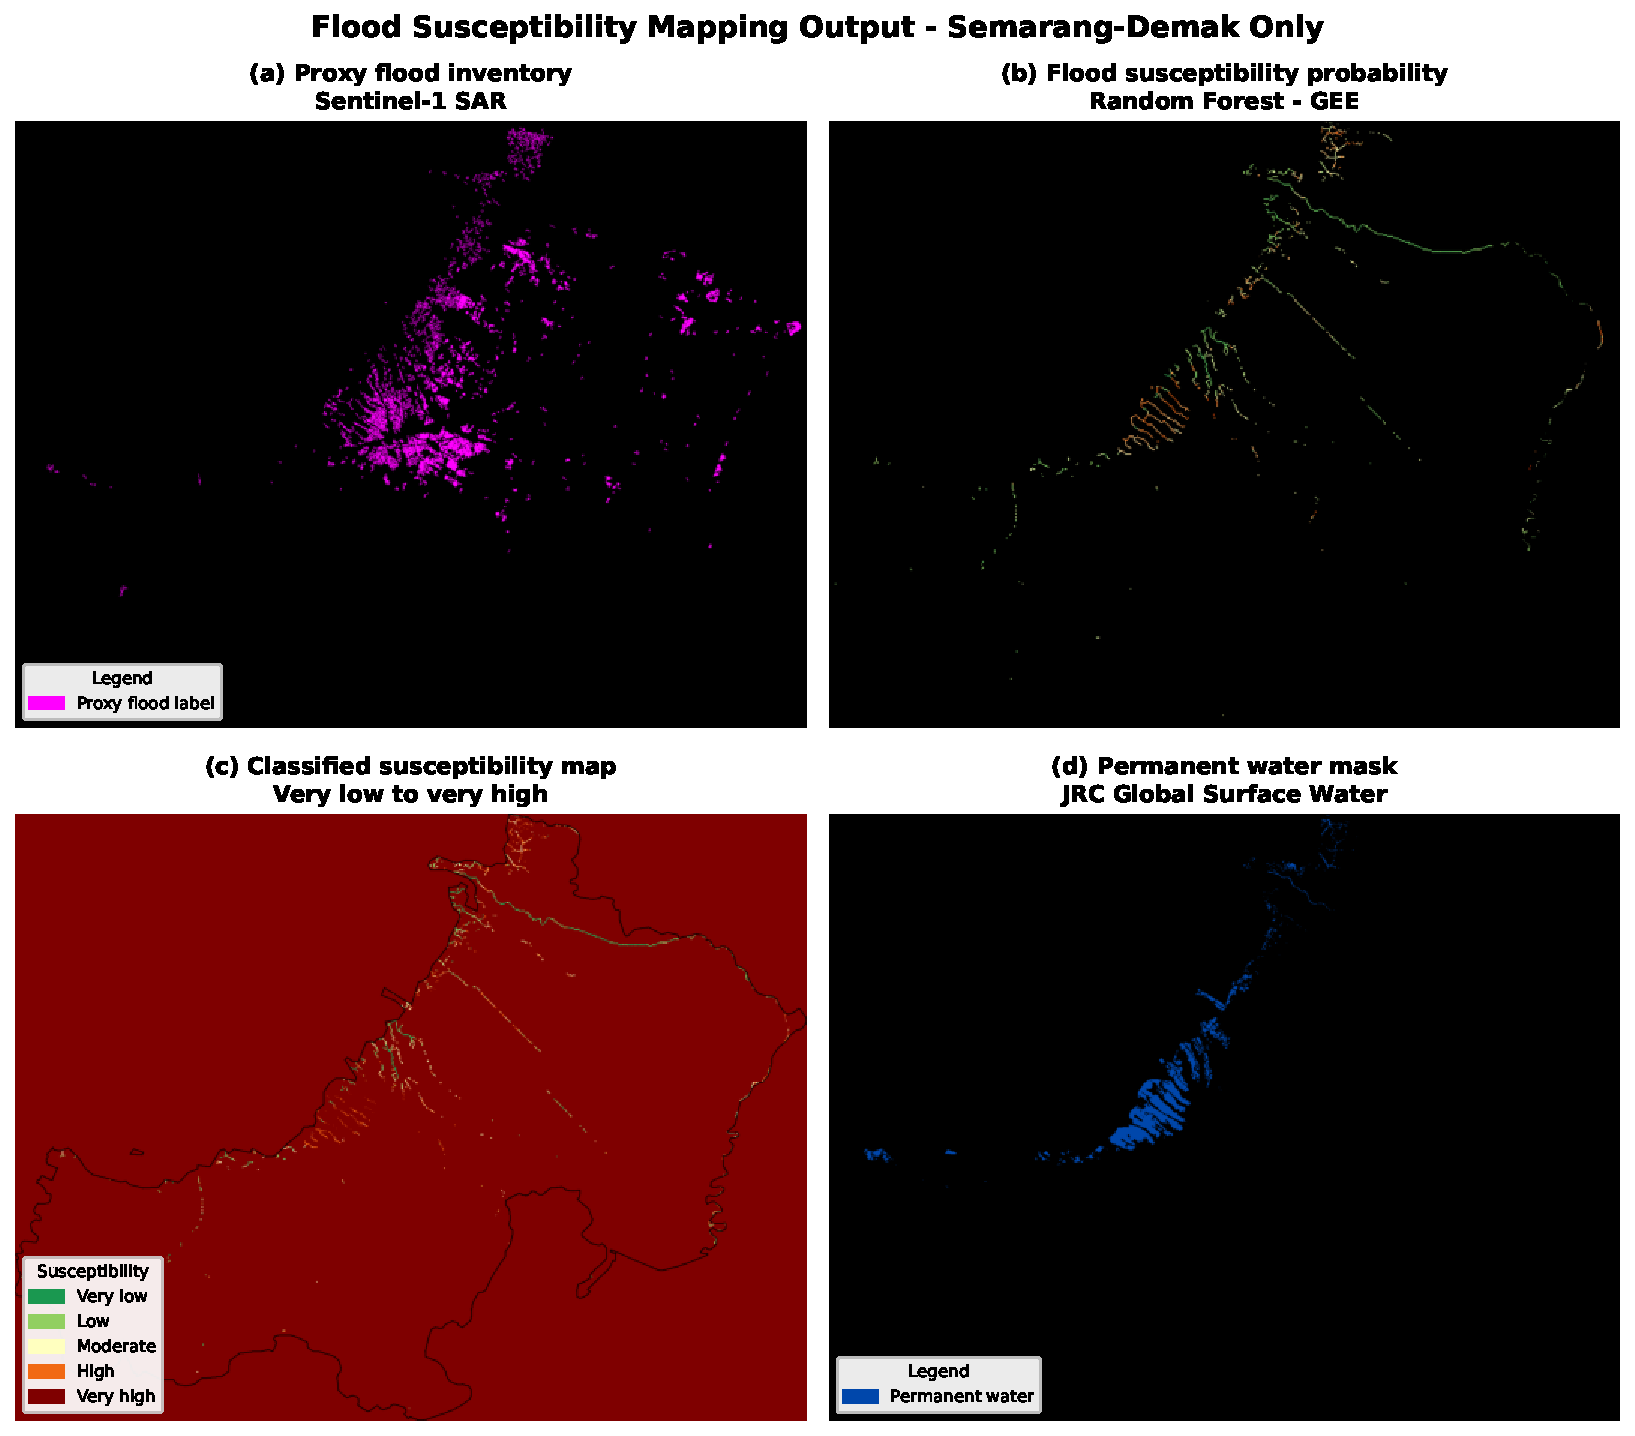
\includegraphics[width=0.55\textwidth]{figures_pdf/image9}
\caption{Final flood susceptibility mapping output for the Semarang-Demak
coastal area. Source: Random Forest raster implementation in Google Earth
Engine.}
\label{fig:susceptibility-map}
\end{figure}
 
\begin{figure}[htbp]
\centering
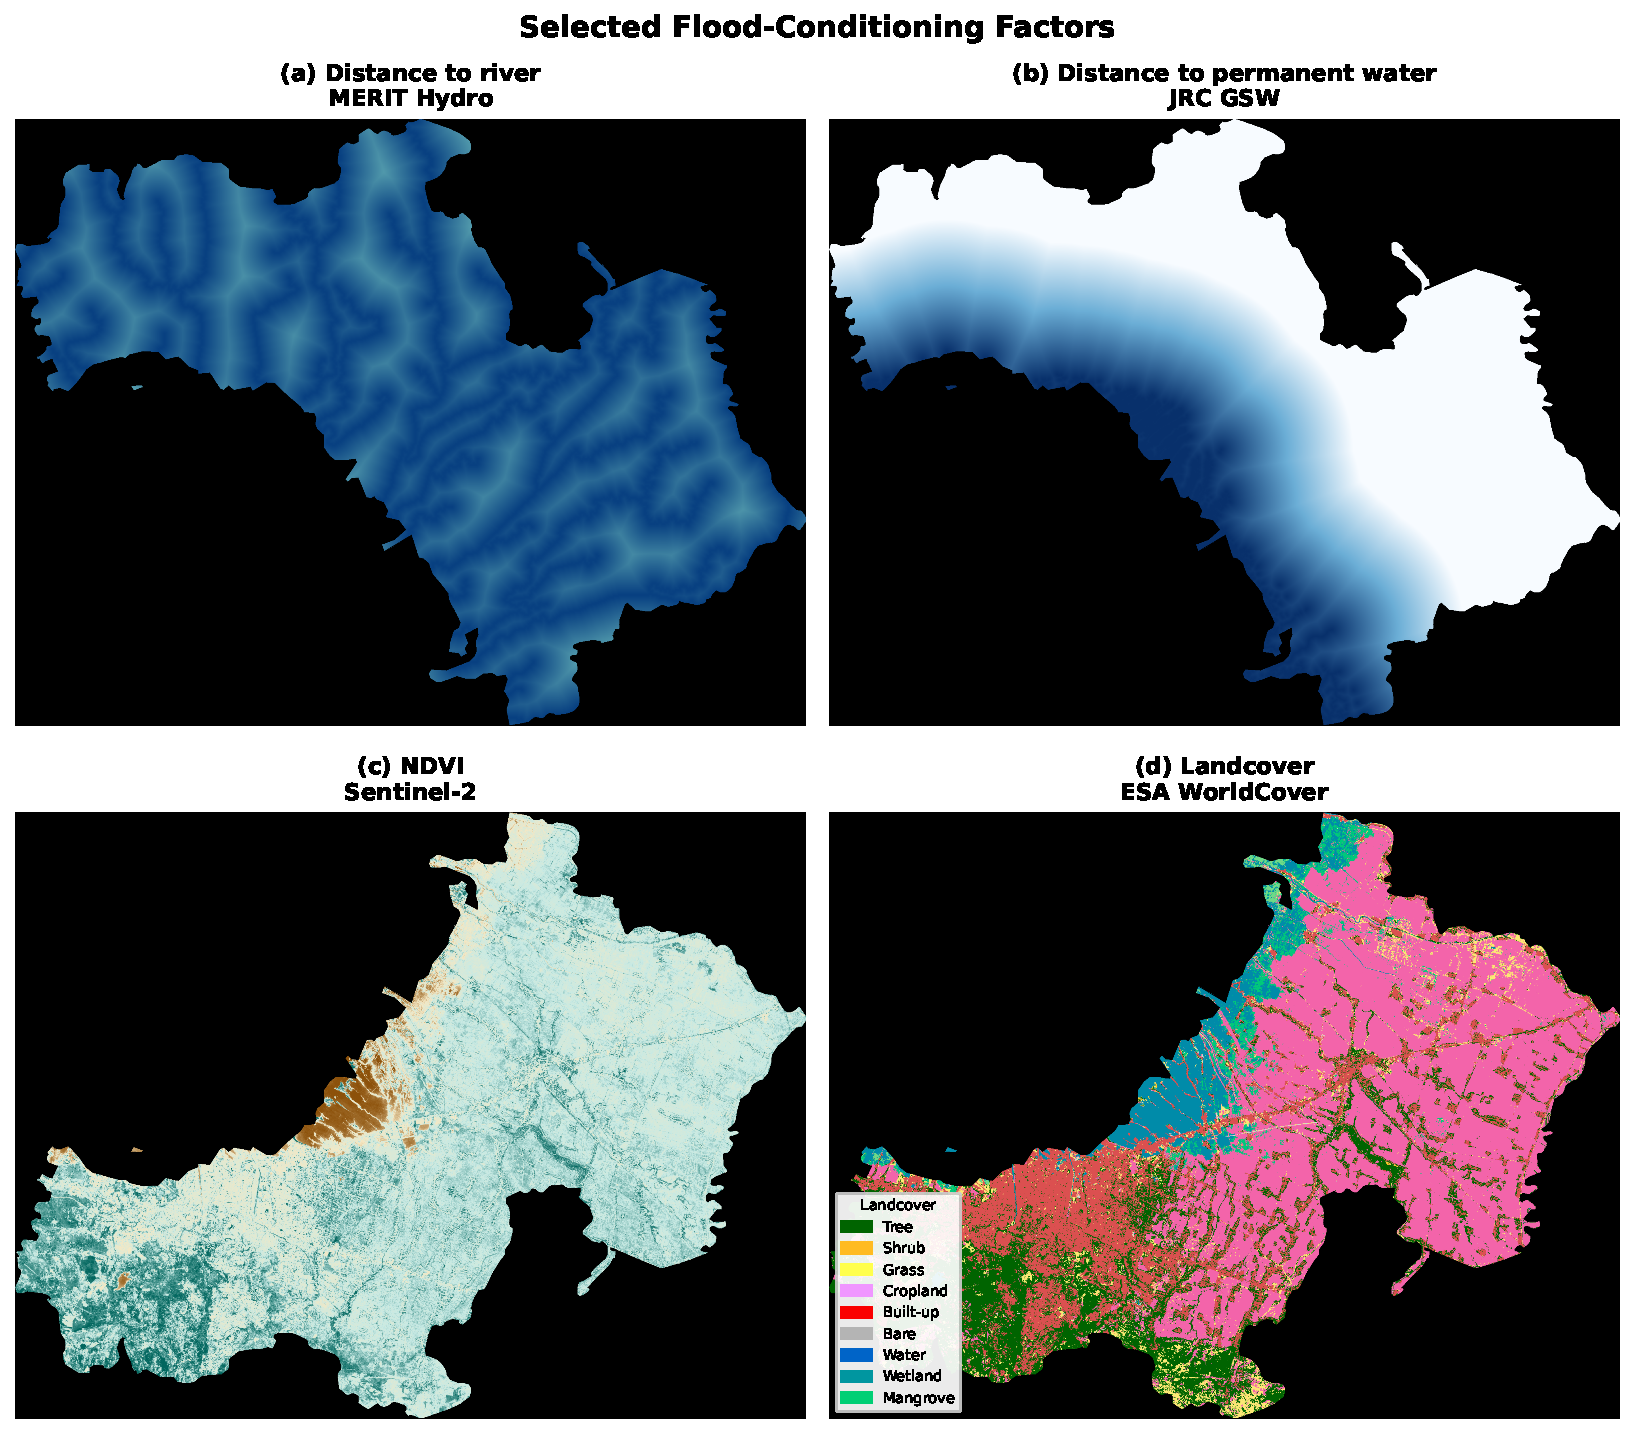
\includegraphics[width=0.55\textwidth]{figures_pdf/image10}
\caption{Selected flood-conditioning factors used to support spatial
interpretation. Source: processed geospatial predictors from Google Earth
Engine.}
\label{fig:conditioning-factors}
\end{figure}
 
The final susceptibility map indicates that higher susceptibility classes are
concentrated in zones that combine water proximity, lowland morphology, wet
surface signals, and built-up pressure. This pattern is consistent with the
coastal-urban flood mechanism of Semarang-Demak. Areas close to permanent water
or drainage features can receive concentrated runoff or experience limited
drainage capacity, while built-up zones may increase impervious surfaces and
reduce infiltration.
 
The map should not be read as a real-time forecast. It represents spatial
similarity to previously detected flooded pixels under the selected predictor
conditions. Therefore, a high-susceptibility pixel does not necessarily mean
that flooding occurred at that exact location on the selected date. Instead, it
indicates that the location has geospatial characteristics resembling
flood-labelled samples. This distinction is central to susceptibility mapping
and prevents overinterpretation of the probability values as event-specific
inundation certainty.
 
The classified map is useful for communicating broad susceptibility gradients,
but the continuous probability map retains more analytical information. The
five-class map can support planning communication, while the probability surface
is more appropriate for technical prioritization because it preserves subtle
spatial differences.
 
%==================================

\FloatBarrier

%==================================
\section{Discussion}\label{discussion}

\subsection{Comparative Performance of the Ensemble Models}\label{comparative-performance}

The comparative results show that all seven ensemble models were able to discriminate between flood and non-flood samples derived from the Sentinel-1-based flood inventory. Random Forest achieved the highest ROC-AUC (0.852) and F1-score (0.816), followed by the Stacking Ensemble (ROC-AUC = 0.850; F1-score = 0.804) and CatBoost (ROC-AUC = 0.849; F1-score = 0.804). XGBoost, LightGBM, ExtraTrees, and Gradient Boosting produced slightly lower ROC-AUC values of 0.842, 0.836, 0.835, and 0.831, respectively. The substantial overlap among the ROC curves further indicates that the predictive behaviour of the evaluated models was broadly similar.

Although Random Forest obtained the highest values for the principal discrimination metrics, the differences among the leading models were relatively small. Therefore, the results should not be interpreted as evidence that Random Forest is universally superior to other ensemble approaches. Instead, its performance indicates a marginal advantage under the present predictor configuration, sampling design, and Sentinel-1-derived flood labels. The statistical comparisons in Section \ref{spatial-cv-results} formalize this reading: Random Forest is statistically inseparable from the stacking ensemble, CatBoost, XGBoost, and LightGBM, and holds only a small margin over the two lowest-ranked models, so the model ranking should be treated as descriptive rather than decisive.

The normalized confusion matrices provide additional insight into this difference. Random Forest correctly classified approximately 93\% of the flood-labelled test samples, resulting in the highest flood recall among the evaluated models, although this was accompanied by a non-flood recall of approximately 65\%. Consequently, its practical advantage is more appropriately interpreted as a relatively stronger ability to identify flood-labelled samples rather than as substantial overall superiority. This distinction is important because the choice of the best-performing model may depend on whether the application prioritizes sensitivity to flood-labelled locations or balanced discrimination between flood and non-flood classes.

The relatively close performance of the ensemble models also provides an important basis for interpreting the subsequent predictor analysis. The convergence of ROC-AUC values suggests that the principal spatial signal contained in the multi-source predictor dataset can be learned by different tree-based ensemble algorithms. Accordingly, the SHAP analysis is not interpreted as evidence that the environmental relationships are unique to Random Forest, but rather as an examination of the environmental information that contributes to the predictions of the selected model. Nevertheless, model performance and predictor importance remain conditional on the present dataset and should not be generalized directly to other flood environments without independent validation.

\subsection{Dominant Role of Permanent-Water Proximity and Antecedent Rainfall}\label{dominant-role-water-rainfall}

The SHAP analysis identifies distance to permanent water (\texttt{dist\_perm\_water}) as the most influential predictor, with the largest mean absolute SHAP value (approximately 0.058). Derived from JRC Global Surface Water, this variable represents the spatial relationship between locations and persistent surface-water features. Its high contribution indicates that the spatial configuration of persistent water contains substantial information for distinguishing flood-labelled from non-flood samples. This interpretation is physically plausible in the Semarang-Demak coastal environment, where rivers, drainage features, ponds, and other persistent water surfaces form interconnected components of a low-lying hydrological landscape. Previous flood susceptibility studies have likewise identified distance or spatial relationships to water bodies as important predictors of flood-prone conditions \cite{Costache2024, Rahimi2026, Glcan2026}.

However, the direction of the SHAP relationship requires particular caution. Higher values of \texttt{dist\_perm\_water} are generally associated with positive SHAP values, whereas lower values tend to occur toward the negative side of the SHAP axis. Therefore, the result does not support a simple interpretation that locations closer to permanent water are necessarily more susceptible to flooding.

\begin{figure}[htbp]
\centering
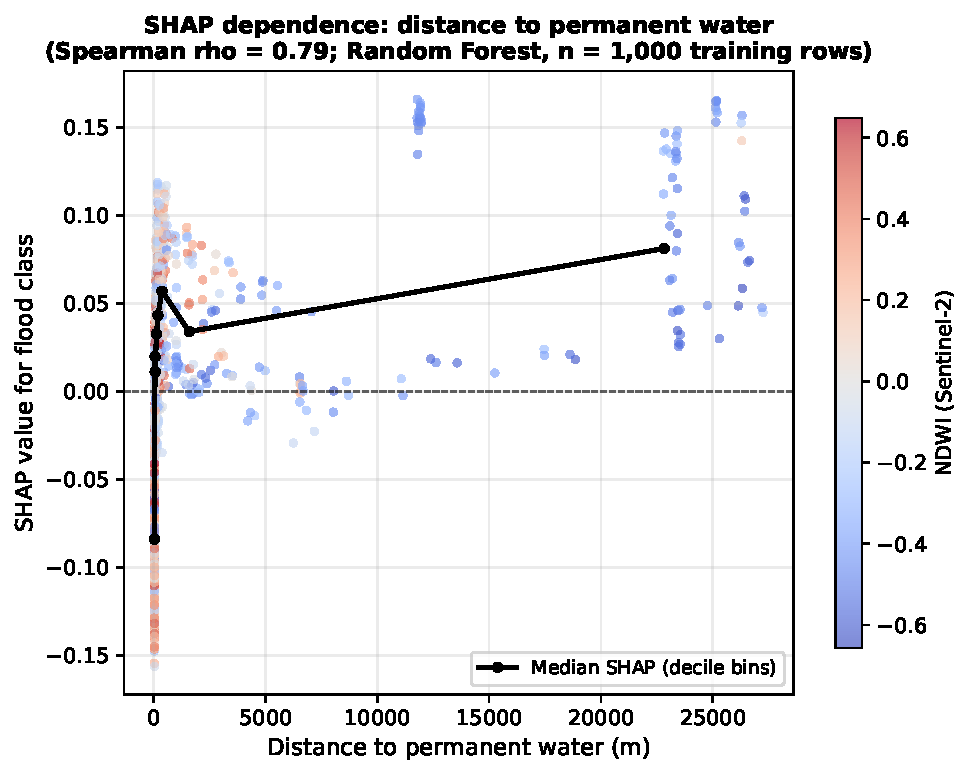
\includegraphics[width=0.6\textwidth]{figures_pdf/image12}
\caption{SHAP dependence plot for distance to permanent water (Random Forest,
1{,}000 training rows). Points are individual samples coloured by NDWI; the
black line and band show the decile-binned median and interquartile range of
the SHAP value. The relationship is strongly non-monotonic: samples within the
first distance bin (median $\approx 30$~m) receive clearly negative SHAP
values, while all farther bins shift toward positive contributions.}
\label{fig:dependence-dist-water}
\end{figure}

The dependence plot in Figure \ref{fig:dependence-dist-water} makes this
pattern explicit. The binned median SHAP value is negative (approximately
$-0.08$) for the closest decile at roughly 30~m from permanent water, rises
steeply across the next bins to approximately $+0.01$ to $+0.06$ at distances of
60~m to 370~m, and
remains positive but more dispersed at larger distances, with an overall
Spearman correlation of $\rho = 0.79$ between the variable and its SHAP value.
The direction is therefore the opposite of the naive distance-decay expectation,
and the most plausible explanation lies in how the training labels were
constructed. Permanent water is explicitly excluded from the flood label, and
the sampling grid starts at the edge of the permanent-water mask; the pixels
nearest to permanent water are therefore frequently narrow shoreline bands that
remain unlabelled even when occasionally inundated, so the model learns to
treat the immediate shoreline fringe as relatively less flood-like than the
low-lying ground slightly farther away. In addition, the negative-SHAP closest
bin coincides with higher NDWI values (Figure \ref{fig:dependence-dist-water},
colour scale), indicating persistent surface moisture rather than event
inundation. The high SHAP importance of \texttt{dist\_perm\_water} hence indicates that the spatial arrangement of persistent water features provides contextual information for the classification. This apparently non-monotonic or counter-intuitive relationship may reflect the fact that persistent water features are spatially associated with broader drainage, pond, coastal, and land-use configurations rather than functioning solely as direct sources of inundation. It may also partly reflect the spatial structure of the Sentinel-1-derived flood inventory itself. Thus, the predictor should be interpreted as a spatial contextual variable rather than as direct evidence of channel overtopping or a causal effect of water proximity.

Antecedent rainfall was the second major source of predictive information. The 30-day rainfall variable (\texttt{rain\_30d}) ranked second, with a mean absolute SHAP value of approximately 0.042, whereas 7-day rainfall (\texttt{rain\_7d}) ranked fourth at approximately 0.031. Higher values of both variables generally occur toward positive SHAP values, indicating that greater accumulated rainfall tends to be associated with predictions of the flood class. This relationship is physically plausible because accumulated precipitation can contribute to antecedent wetness and hydrological loading, potentially reducing the capacity of the landscape to accommodate additional rainfall and increasing the likelihood of surface water accumulation \cite{Zhao2025, Alcntara2025}. Importantly, this interpretation represents a plausible physical mechanism rather than a directly measured process, because the present model does not explicitly measure groundwater level, soil moisture, or infiltration capacity.

The stronger contribution of 30-day rainfall compared with 7-day rainfall is particularly noteworthy. The result suggests that precipitation accumulated over a longer antecedent period contains more discriminatory information than rainfall over the shorter temporal window considered here. This may indicate that pre-event hydrological conditions are relevant to the spatial distribution of the flood-labelled samples, rather than the observed flood pattern being associated solely with immediate rainfall forcing. Similar emphasis on antecedent precipitation or cumulative rainfall has been reported in flood susceptibility and flood modelling studies \cite{Zhao2025}.

Nevertheless, the present result should not be interpreted as evidence that long-term rainfall accumulation is universally more important than short-duration rainfall. In Semarang-Demak, where flooding may arise through interacting rainfall, drainage, riverine, and coastal processes, the relative contribution of rainfall accumulation is likely to depend on the specific flood event and its antecedent conditions.

\subsection{Contribution of Surface Characteristics from Sentinel-2}\label{contribution-sentinel2}

NDVI was the third most influential predictor, with a mean absolute SHAP value of approximately 0.036. Higher NDVI values are predominantly associated with negative SHAP contributions, whereas lower values more frequently occur toward positive SHAP values. This indicates that locations characterized by lower vegetation-index values tend to be associated with higher predicted flood susceptibility within the present model. A plausible physical interpretation is that vegetation-related surface conditions can differentiate areas with greater vegetation cover from more intensively developed, sparsely vegetated, or water-influenced surfaces. Vegetated surfaces can enhance infiltration and influence runoff processes, whereas impervious or sparsely vegetated surfaces may permit greater generation of surface runoff \cite{Aniramu2026}.

The observed negative contribution of high NDVI is broadly consistent with previous flood susceptibility studies reporting that vegetation-related indices can contribute to the discrimination of flood-prone areas \cite{Rahimi2026}. However, NDVI should not be interpreted as a direct causal determinant of flooding. The index is a remotely sensed proxy for vegetation-related surface characteristics and can also vary with land-cover type, seasonal vegetation condition, moisture, and other environmental factors. Consequently, its SHAP contribution is better interpreted as evidence that vegetation-related surface conditions contain useful spatial information for distinguishing the Sentinel-1-derived flood labels. In Semarang-Demak, this information is particularly relevant because agricultural and vegetated surfaces coexist with expanding built-up areas and water-influenced coastal landscapes.

The water-sensitive indices derived from Sentinel-2 also contributed meaningfully to the model. MNDWI and NDWI obtained mean absolute SHAP values of approximately 0.026 and 0.023, respectively, and higher values generally occurred toward positive SHAP contributions. This behaviour is consistent with the role of these indices in representing water-related and moisture-sensitive surface characteristics. Higher index values are generally associated with stronger indications of surface-water presence, while MNDWI can improve the discrimination of water features from built-up and vegetated surfaces \cite{Bhatt2026}. This spectral sensitivity may therefore provide additional information for distinguishing flood-labelled from non-flood locations. Nevertheless, the indices should not be interpreted as direct measurements of flood occurrence because their values can also reflect persistent surface water and other water-influenced land-cover conditions.

The contribution of these Sentinel-2 indices is particularly relevant because the flood inventory was derived from Sentinel-1 SAR. Their predictive contribution therefore provides complementary optical surface information associated with the spatial distribution of the SAR-derived flood labels. This does not constitute independent validation of the Sentinel-1 inventory, because the Sentinel-2 variables are predictors within the same supervised modelling framework. Rather, the result indicates that the flood-labelled spatial pattern contains information that is also reflected in optical characteristics of the surface.

NDBI produced a mean absolute SHAP value of approximately 0.025, indicating a meaningful contribution to the model predictions. However, the SHAP distribution does not show a clear monotonic relationship between NDBI values and SHAP contributions, as both relatively low and high NDBI values occur across positive and negative SHAP values. This pattern suggests that the contribution of built-up intensity is not uniform across the study area and may be context-dependent. Because NDBI provides information related to built-up and impervious surface characteristics, variations in NDBI may reflect differences in surface conditions associated with infiltration and runoff processes \cite{Kebede2022, Shukuru2024}. In the Semarang-Demak setting, this relationship is particularly relevant because developed areas coexist with low-lying coastal terrain and interconnected drainage systems. Nevertheless, NDBI should be interpreted as a proxy for built-up surface characteristics rather than as direct evidence that urbanization alone caused the observed inundation.

\subsection{Hydrological Connectivity and Upstream Drainage Conditions}\label{hydrological-connectivity}

The hydrological variables derived from MERIT Hydro provided another important component of the predictive signal. Upstream drainage area (\texttt{upa\_log}) ranked fifth, with a mean absolute SHAP value of approximately 0.030, while river width and distance to river each had mean absolute SHAP values of approximately 0.024. These variables represent different dimensions of hydrological structure: upstream drainage area describes the contributing area of the drainage network, whereas river width and distance to river represent the spatial relationship between locations and river channels.

Importantly, the SHAP directions were not uniform across these variables. Higher \texttt{upa\_log} values were predominantly associated with negative SHAP values, while lower values tended to be associated with positive contributions. Similarly, higher river-width values were more frequently distributed toward negative SHAP values, whereas larger distance-to-river values tended to occur more frequently on the positive side of the SHAP axis. These patterns indicate that the model did not learn a simple relationship in which greater hydrological connectivity uniformly corresponds to greater flood susceptibility. Instead, the contribution of hydrological variables appears to depend on their spatial configuration and interaction with other environmental conditions.

This finding is consistent with the understanding that flood susceptibility is not determined solely by distance from a river. Previous studies have emphasized the roles of drainage configuration, contributing area, channel characteristics, and the interaction between surface conditions and hydrological pathways in determining inundation patterns \cite{Costache2024, jeddah2025, Alcntara2025, Rahimi2026}. In a coastal environment, water may be redistributed through interconnected rivers, drainage channels, ponds, and low-lying surfaces, meaning that the effect of a hydrological variable can vary spatially. Therefore, the combined contribution of \texttt{upa\_log}, river width, and distance to river is more informative than interpreting any one of these variables in isolation.

The relatively high contribution of \texttt{upa\_log} compared with elevation and slope further suggests that hydrological structure provides predictive information beyond simple terrain descriptors. One possible explanation is that the drainage network captures aspects of water connectivity that are not fully represented by elevation or slope alone. However, this interpretation remains inferential because the present predictor set does not explicitly represent hydraulic infrastructure such as embankments, flood gates, pumping systems, or drainage capacity. The observed SHAP patterns should therefore be interpreted as evidence of spatial association with hydrological structure rather than direct evidence of a particular hydraulic mechanism.

\subsection{Topography and the Characteristics of a Low-Lying Coastal Environment}\label{topography-coastal-environment}

Slope and elevation were less influential than permanent-water proximity, antecedent rainfall, NDVI, and the principal hydrological variables, with mean absolute SHAP values of approximately 0.020 and 0.013, respectively. Aspect had an even smaller contribution. These results do not indicate that topography is physically unimportant for flooding. Rather, they suggest that, within the environmental and spatial conditions represented by the present Semarang-Demak dataset, simple terrain descriptors provide less discriminatory information than several variables describing water-related conditions and surface characteristics.

The SHAP directions are nevertheless physically plausible: higher slope and elevation values generally tend to contribute negatively, whereas lower values are more frequently associated with positive contributions. Lower and flatter locations can provide greater potential for water accumulation, and this relationship has been widely recognized in flood susceptibility modelling \cite{Alcntara2025, Rahimi2026}. However, the relatively modest SHAP magnitudes indicate that elevation and slope alone do not adequately distinguish the flood-labelled locations in the present case.

One possible explanation is the low-relief character of the Semarang-Demak coastal zone. When the study area is dominated by relatively low-lying terrain, the spatial variability of elevation and slope may provide less discriminatory information than variables that capture water proximity, rainfall accumulation, and hydrological connectivity. In this context, a lower SHAP importance for elevation does not imply that elevation is irrelevant to flood processes. Instead, it indicates that its incremental predictive contribution is comparatively limited within this particular study area and predictor configuration. This distinction is important when comparing the present results with studies conducted in areas characterized by larger topographic gradients, where elevation and slope may have greater discriminatory power \cite{Costache2024, Rahimi2026}.

\subsection{Land-Cover Variables and Categorical Predictor Interpretation}\label{landcover-interpretation}

The ESA WorldCover land-cover variables contributed less strongly than the principal continuous environmental predictors. Among the land-cover variables, \texttt{lc\_90} showed the largest mean absolute SHAP contribution, followed by \texttt{lc\_95}, \texttt{lc\_40}, \texttt{lc\_80}, \texttt{lc\_30}, and \texttt{lc\_10}, while HAND produced the smallest contribution in the SHAP ranking. These results indicate that the model relied more strongly on continuous measures of water proximity, rainfall, surface condition, and hydrological structure than on the individual land-cover categories.

The categorical nature of the WorldCover variables requires particular caution in interpreting the SHAP results. Unlike rainfall, elevation, or distance, the numerical class identifiers do not represent an ordered physical gradient. Therefore, a positive or negative SHAP value associated with a land-cover category should not be interpreted as evidence that increasing the numerical class value increases or decreases flood susceptibility. Instead, the land-cover variables should be interpreted in terms of how much information each encoded category contributes to model discrimination. This approach avoids assigning an artificial ordinal meaning to categorical land-cover classes.

The relatively smaller contribution of the land-cover variables also does not imply that land cover is irrelevant to flooding. Rather, the result suggests that much of the spatial differentiation captured by the model can be represented more directly through continuous environmental gradients such as water proximity, rainfall accumulation, vegetation characteristics, built-up intensity, and hydrological structure. In Semarang-Demak, where different land-cover classes occur within a strongly interconnected coastal environment, these continuous variables may capture spatial contrasts that are not fully represented by categorical land-cover labels alone.

\subsection{Spatial Interpretation of the Predicted Susceptibility}\label{spatial-interpretation}

The final susceptibility map generated using Random Forest provides a spatial representation of the environmental relationships learned from the multi-source predictor dataset. When interpreted together with the Sentinel-1-derived flood inventory and the permanent-water information, the map should be understood as a generalization of the environmental characteristics associated with flood-labelled pixels to the broader study area. It is therefore not a direct reproduction of the observed Sentinel-1 flood extent.

The spatial pattern is consistent with the SHAP interpretation in that the model integrates information from permanent-water proximity, antecedent rainfall, hydrological structure, vegetation-related surface conditions, and built-up intensity. The resulting susceptibility surface therefore represents the combined contribution of multiple environmental dimensions rather than the influence of a single conditioning factor. This is particularly useful for a coastal region such as Semarang-Demak, where flood-related processes can vary spatially across urban, agricultural, drainage, riverine, and coastal environments.

Nevertheless, the susceptibility map should be interpreted as a relative representation of environmental similarity to the flood-labelled samples rather than as a deterministic flood forecast. A high susceptibility value indicates that the environmental conditions at a location resemble those associated with the Sentinel-1-derived flood labels. It does not mean that the location must be inundated during every rainfall event, nor does the predicted value represent a directly measured flood probability, depth, or duration. This distinction is particularly important because the supervisory target is a remotely sensed proxy for inundation rather than a field-verified measurement of hydrodynamic flood characteristics.

\subsection{Implications of Excluding Land Subsidence and Tidal Dynamics}\label{discussion-subsidence-tidal}

The present predictor set deliberately represents rainfall-runoff and
hydrological-proximity mechanisms, and it does not include land subsidence or
tidal stage. This omission is a practical necessity rather than a judgement
that these processes are unimportant. No consistent, event-period raster
products exist for either process at the 30~m modelling scale: land-subsidence
estimates for Semarang-Demak derive from intermittent PS-InSAR campaigns
\parencite{abidin2015}, and tidal conditions vary hourly and would require
in-situ gauge records or tide models that cannot currently be sampled as
per-pixel features inside Google Earth Engine. Because the susceptibility
target is a single-event inventory, static or slowly varying proxies for these
processes would also be difficult to interpret unambiguously.

Their absence nevertheless conditions what the model can and cannot express.
Land subsidence and tidal flooding in Semarang-Demak operate largely through
the same pathways the model does capture: they raise low-lying ground toward
the water table, expand the footprint of permanent and semi-permanent water,
and intensify drainage congestion. Part of their influence is therefore
absorbed, in a time-averaged sense, by the variables the model does observe,
notably elevation, HAND, distance to permanent water, and the coastal
land-cover classes. What the model cannot express is the temporal dynamics:
it cannot distinguish a location that floods because of heavy antecedent
rainfall from one flooded primarily by a spring tide, nor can it project
forward as subsidence progressively enlarges the exposed area. Consequently,
the susceptibility map should be read as a rainfall-runoff-and-proximity
assessment of present-day conditions, not as a total coastal-hazard map. Areas
subject to rapid subsidence or frequent rob flooding may be underrepresented
if their surface characteristics resemble those of non-subsiding inland areas,
and the map should be intersected with subsidence-rate and tidal-inundation
layers before being used for coastal-zone planning or adaptation decisions.

\subsection{Implications and Limitations of the Sentinel-1-Based Supervised Framework}\label{implications-limitations}

The results demonstrate the potential of combining a Sentinel-1-derived flood inventory with multi-source geospatial predictors for supervised flood susceptibility modelling in a data-limited coastal setting. The framework provides a way to transform an event-derived flood inventory into a spatial learning target and relate the resulting flood-labelled pattern to environmental variables that extend beyond the observed inundation footprint. The relatively similar performance of the evaluated ensemble models further suggests that the underlying spatial signal is sufficiently consistent to be learned by multiple tree-based approaches.

At the same time, the findings should not be interpreted as establishing a universally optimal model or a universal hierarchy of flood-conditioning factors. Random Forest performed marginally better than the other models for the present dataset, but the difference in ROC-AUC among the leading models was less than 0.01. Likewise, the SHAP ranking represents the relative contribution of predictors within this particular modelling framework and study area. These rankings may change under different flood events, predictor configurations, sampling strategies, or environmental settings.

Several limitations should also be considered. First, the Sentinel-1-derived flood inventory is a remotely sensed proxy and may contain uncertainties associated with SAR backscatter behaviour, surface scattering, permanent-water masking, and the selected change-detection threshold. Such uncertainties can propagate into the supervised learning stage. Consequently, the susceptibility relationships learned by the models may partly reflect characteristics of the particular flood event used to construct the supervisory labels rather than stable relationships applicable to all flood events.

Second, because the observations are spatially distributed, the random train-test split benefits from spatial autocorrelation between neighbouring samples. The spatial block cross-validation performed in this study quantifies this effect explicitly: when entire $\sim$10~km blocks are held out, cross-validated ROC-AUC falls from 0.82--0.84 to 0.56--0.61 across all models (Section \ref{spatial-cv-results}). The headline metrics in Table \ref{tab:model-performance} should therefore be read as within-domain discrimination estimates, while the spatially validated figures represent a more conservative bound on generalization to geographically distinct locations. Future work should extend this design to multi-event inventories, where blocks from different flood events can serve as genuinely independent evaluation units.

Third, several important coastal flood processes are not explicitly represented in the current predictor set. Tidal conditions, land subsidence, hydraulic infrastructure, and other dynamic coastal processes can influence inundation patterns in Semarang-Demak but are not directly captured by the present framework. Previous research has highlighted the importance of land subsidence in the coastal Semarang-Demak environment \parencite{abidin2015}. Incorporating such dynamic variables in future multi-event studies could provide a more complete representation of the physical processes underlying coastal flooding.

Future research should therefore combine multi-event Sentinel-1 flood inventories with spatially independent validation across events and additional coastal predictors, including tidal conditions and land-subsidence information. Such extensions would allow researchers to test whether the predictor relationships identified in the present study remain stable across different flood events and environmental conditions. They could also help distinguish relationships that are specific to the spatial structure of a particular flood inventory from those that represent more transferable flood-susceptibility characteristics. In this way, the Sentinel-1-based supervised framework can serve as a basis for progressively more generalizable flood susceptibility assessment in Indonesian coastal environments.
%==================================
\section{Conclusion}\label{conclusions}

The findings demonstrate that flood susceptibility in the Semarang-Demak coastal area is primarily associated with the spatial and environmental characteristics of water-related conditions, antecedent rainfall, vegetation, drainage structure, and developed surfaces. SHAP analysis identified distance to permanent water as the most influential predictor, followed by antecedent rainfall, NDVI, upstream drainage area, MNDWI, NDBI, river width, distance to river, and NDWI. These results indicate that the spatial pattern of flood-labelled locations is not governed by a single conditioning factor, but rather reflects the combined information contained in water proximity, rainfall accumulation, hydrological connectivity, surface characteristics, and built-up conditions. Importantly, the SHAP results represent predictor contributions to the model predictions and should not be interpreted as direct evidence of causal relationships.

Among the evaluated ensemble models, Random Forest achieved the strongest overall performance, with a ROC-AUC of 0.852 and an F1-score of 0.816. However, DeLong tests and paired bootstrap comparisons showed that Random Forest is statistically inseparable from the other leading models (all $p \geq 0.07$), with only marginal separation from the two lowest-ranked models, so it should be regarded as the best point estimate under the present configuration rather than a statistically distinguishable winner. Five-fold spatial block cross-validation additionally showed that random-split estimates are optimistic for spatial generalization, with cross-validated ROC-AUC falling to the 0.56--0.61 range when $\sim$10 km blocks are held out. The model's relatively high flood recall further indicates its ability to identify flood-labelled samples, although this was accompanied by a lower recall for the non-flood class.

The resulting susceptibility map shows that higher susceptibility is concentrated in coastal zones characterized by combinations of water-related conditions, lowland morphology, wet surface signals, and built-up pressure. The map therefore provides a spatial screening representation of environmental similarity to the Sentinel-1-derived flood-labelled samples rather than a deterministic prediction of inundation during future rainfall events. Its primary value is to support the identification and prioritization of areas requiring further flood-risk assessment and management.

Overall, this study demonstrates the potential of transforming Sentinel-1-derived flood detection into a supervised and explainable flood susceptibility framework for data-limited coastal environments. The integration of multi-source geospatial predictors, comparative ensemble learning, and SHAP interpretation provides both predictive and spatially interpretable information for the Semarang-Demak coastal area. Nevertheless, the findings remain conditional on the selected flood event, Sentinel-1-derived supervisory labels, predictor configuration, and validation strategy. Future research should incorporate multi-event flood inventories, spatially independent validation, and additional dynamic coastal predictors such as tidal conditions, land subsidence, and hydraulic infrastructure to evaluate the transferability and generalizability of the identified susceptibility relationships.
 
 %==================================
\section*{Data Availability}
The balanced training sample (1,870 rows), the raw sample, and the exact train-test split assignment (seed 42) are available as a public Kaggle dataset at \url{https://www.kaggle.com/datasets/nxtirfan/semarang-demak-flood-training-data}. All machine-readable outputs of the revised analyses---test predictions, DeLong/bootstrap tables, cross-validation summaries, fold assignment, correlation matrices, and SHAP summaries---are available at \url{https://www.kaggle.com/datasets/nxtirfan/semarang-demak-flood-training-and-results}. The complete analysis notebook, which reproduces every revised statistic from the CSV data without requiring Google Earth Engine access, is available as a Kaggle kernel at \url{https://www.kaggle.com/code/nxtirfan/flood-susceptibility-semarang-demak-revision}. The Sentinel-1, Sentinel-2, SRTM, MERIT Hydro, JRC Global Surface Water, CHIRPS, and ESA WorldCover source products were accessed through Google Earth Engine and are publicly available from their respective providers.
 
%==================================
\acknowledg{The authors thank the anonymous reviewers for their constructive
comments and suggestions. Gratitude is also extended to all parties who supported
the data collection and geospatial processing stages of this study.}
 
%==================================
\FloatBarrier
\printbibliography
 
\end{document}

%==================================
\appendix % [Optional]

\section{Supplementary Mathematical Derivations}
\label{Sec:SuppA}
Additional derivations supporting the proposed statistical model.


\end{document}

